% =====================================================================
%  Il tiristore (SCR): funzionamento e fisica del dispositivo
%  Documento in italiano, terminologia tecnica in inglese
%  Compilare con pdflatex (2 passate)
% =====================================================================
\documentclass[11pt,a4paper]{article}
\usepackage[utf8]{inputenc}
\usepackage[T1]{fontenc}
\usepackage{textcomp}
\usepackage[sc]{mathpazo}
\linespread{1.04}
\usepackage[margin=2.3cm]{geometry}
\usepackage{amsmath,amssymb}
\usepackage{siunitx}
\usepackage{booktabs}
\usepackage{array}
\usepackage{caption}
\usepackage{subcaption}
\usepackage{tikz}
\usepackage{circuitikz}
\usepackage{pgfplots}
\pgfplotsset{compat=1.18}
\usetikzlibrary{arrows.meta,calc,positioning,decorations.pathreplacing,patterns}
\usepackage{microtype}
\usepackage[colorlinks=true,linkcolor=blue!50!black,citecolor=blue!50!black,urlcolor=blue!50!black]{hyperref}

% --- Nomi italiani (babel-italian non disponibile) ---
\renewcommand{\contentsname}{Indice}
\renewcommand{\figurename}{Figura}
\renewcommand{\tablename}{Tabella}
\renewcommand{\refname}{Bibliografia}
\renewcommand{\abstractname}{Sommario}

\sisetup{output-decimal-marker={,},per-mode=symbol,range-phrase={\text{--}},range-units=single,list-units=single}
\captionsetup{font=small,labelfont=bf,width=0.92\textwidth}

% --- macro ---
\newcommand{\VAK}{\ensuremath{V_{AK}}}
\newcommand{\IA}{\ensuremath{I_A}}
\newcommand{\IK}{\ensuremath{I_K}}
\newcommand{\IG}{\ensuremath{I_G}}
\newcommand{\IH}{\ensuremath{I_H}}
\newcommand{\IL}{\ensuremath{I_L}}
\newcommand{\VBO}{\ensuremath{V_{BO}}}
\newcommand{\VDRM}{\ensuremath{V_{DRM}}}
\newcommand{\VRRM}{\ensuremath{V_{RRM}}}
\newcommand{\tq}{\ensuremath{t_q}}
\newcommand{\dvdt}{\ensuremath{\mathrm{d}v/\mathrm{d}t}}
\newcommand{\didt}{\ensuremath{\mathrm{d}i/\mathrm{d}t}}
\newcommand{\dd}{\mathrm{d}}
\newcommand{\en}[1]{\emph{#1}}   % termine tecnico inglese

\tikzset{
  layerP/.style={fill=red!20},
  layerPp/.style={fill=red!40},
  layerN/.style={fill=blue!12},
  layerNp/.style={fill=blue!35},
  metal/.style={fill=black!65},
  junc/.style={very thick},
  dim/.style={<->,>=Stealth,thin},
  ax/.style={->,>=Stealth,thick},
}

\title{Il tiristore (SCR):\\ principio di funzionamento e fisica del dispositivo}
\author{Davide Bagnara}
\date{Agosto 2026}

\begin{document}
\maketitle

\begin{abstract}
Questo documento descrive il funzionamento del tiristore (\en{Silicon Controlled Rectifier}, SCR) partendo dalla struttura fisica a quattro strati e dalla fisica dei semiconduttori che ne governa i vari stati: blocco diretto e inverso, innesco, conduzione e spegnimento. Il modello a due transistori viene usato come filo conduttore per collegare i fenomeni microscopici (iniezione di portatori, guadagni di corrente, moltiplicazione a valanga, carica immagazzinata) ai parametri macroscopici che compaiono nei \en{data sheet} (\VBO, \IH, \IL, $\dvdt$, $\didt$, $Q_{rr}$, \tq). Le figure sono disegnate in TikZ e sono di tipo qualitativo: gli ordini di grandezza numerici sono riferiti a tiristori di potenza in silicio per controllo di fase (\en{phase-control thyristor}) nella classe \qtyrange{1}{8}{\kV}.
\end{abstract}

\tableofcontents
\clearpage

% =====================================================================
\section{Introduzione}
% =====================================================================
Il tiristore è il primo dispositivo a semiconduttore di potenza a \en{turn-on} controllato (1957, General Electric, sulla base della struttura p-n-p-n studiata da Moll \en{et al.}~\cite{moll1956}) e resta ancora oggi il componente con la più alta capacità in tensione e corrente per singolo chip: dispositivi \en{press-pack} da \qty{8.5}{\kV} e oltre \qty{5}{\kA}, con correnti di picco di sovraccarico superiori a \qty{100}{\kA}. Le applicazioni tipiche sono i raddrizzatori controllati e i convertitori a commutazione di rete (HVDC-LCC, azionamenti DC, elettrolisi, forni), gli \en{static switch} e i \en{soft starter}, i \en{crowbar} e i circuiti a scarica impulsiva.

Dal punto di vista funzionale il tiristore è un interruttore a tre terminali (anodo A, catodo K, gate G) con tre stati:
\begin{enumerate}
  \item \textbf{blocco inverso} ($\VAK<0$): si comporta come un diodo polarizzato inversamente;
  \item \textbf{blocco diretto} ($\VAK>0$, non innescato): sostiene tensione con una piccola corrente di \en{leakage};
  \item \textbf{conduzione} (\en{on-state}): dopo un impulso di corrente sul gate conduce come un diodo, con caduta di \qtyrange{1}{2.5}{\V}, e il gate perde il controllo. Lo spegnimento avviene solo quando il circuito esterno porta la corrente sotto la \en{holding current}.
\end{enumerate}

Questa asimmetria (accensione comandata, spegnimento affidato al circuito) è la conseguenza diretta della struttura interna: un anello a retroazione positiva fra due transistori bipolari che, una volta chiuso, si sostiene da solo. I capitoli seguenti sviluppano questa idea a partire dalla fisica dei semiconduttori.

% =====================================================================
\section{Struttura del dispositivo}
% =====================================================================
\subsection{Strati, giunzioni e drogaggi}
Il tiristore è una struttura a quattro strati $p^+\,n^-\,p\,n^+$ con tre giunzioni, indicate da anodo a catodo come J1, J2 e J3 (Fig.~\ref{fig:struttura}). I quattro strati hanno funzioni e caratteristiche molto diverse:
\begin{itemize}
  \item \textbf{Emettitore di anodo} $p^+$ (P1): fortemente drogato ($N_A \approx \qtyrange{e18}{e19}{\per\cm\cubed}$), spessore \qtyrange{30}{60}{\um}, ottenuto per diffusione di alluminio o boro. Inietta lacune nella base $n^-$ in conduzione.
  \item \textbf{Base n} $n^-$ (N1): è la regione che sostiene la tensione in entrambe le polarità. Silicio a bassissimo drogaggio ($N_D \approx \qtyrange{5e12}{1e14}{\per\cm\cubed}$), tipicamente ottenuto per trasmutazione neutronica (NTD) per garantire uniformità radiale. Lo spessore $W_N$ va da circa \qty{200}{\um} (\qty{1.6}{\kV}) a oltre \qty{1000}{\um} (\qty{8}{\kV}), con una regola empirica di \qtyrange{80}{120}{\um\per\kV} per dispositivi simmetrici senza \en{field stop}.
  \item \textbf{Base p} $p$ (P2): drogaggio intermedio ($N_A$ di picco \qtyrange{e16}{e17}{\per\cm\cubed}, profilo gaussiano da diffusione), spessore \qtyrange{30}{100}{\um}. È la base del transistor n-p-n, ospita il contatto di gate e fissa la sensibilità di innesco e la robustezza al $\dvdt$.
  \item \textbf{Emettitore di catodo} $n^+$ (N2): molto drogato ($N_D \approx \qty{e20}{\per\cm\cubed}$), sottile (\qtyrange{10}{20}{\um}), diffuso da fosforo. Non è uno strato continuo ma è interdigitato con la base p (\en{cathode shorts}, \S\ref{sec:dvdt}) e con la struttura di gate.
\end{itemize}

\begin{figure}[htbp]
\centering
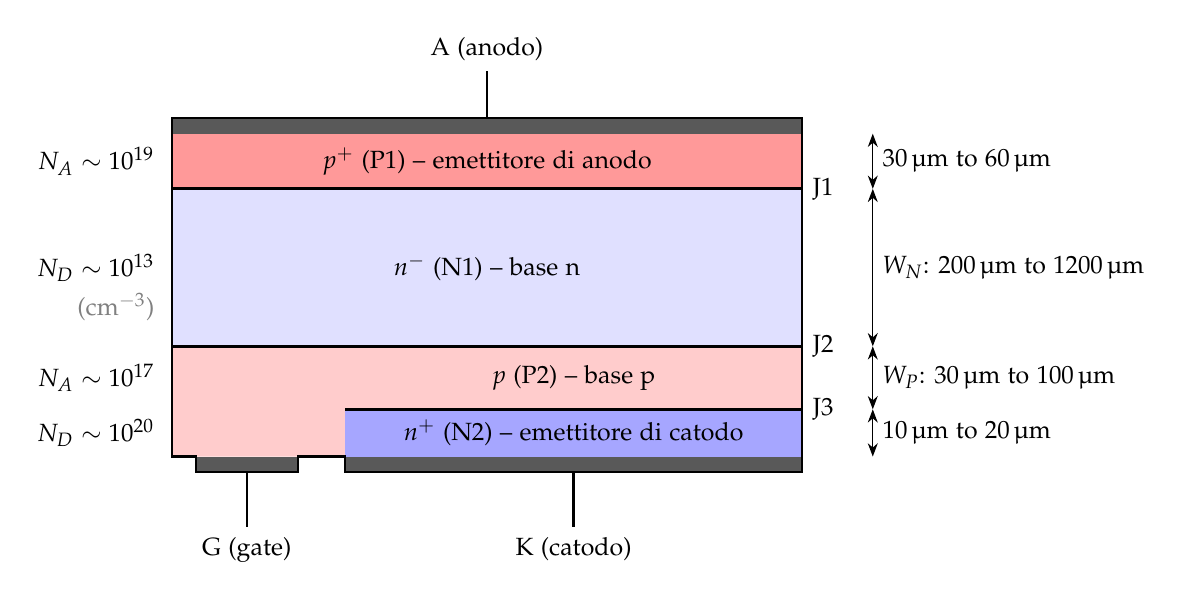
\begin{tikzpicture}[x=1cm,y=1cm,font=\small]
  % strati
  \fill[layerPp] (0,4.0) rectangle (8,4.7);
  \fill[layerN]  (0,2.0) rectangle (8,4.0);
  \fill[layerP]  (0,2.0) -- (8,2.0) -- (8,1.2) -- (2.2,1.2) -- (2.2,0.6) -- (0,0.6) -- cycle;
  \fill[layerNp] (2.2,0.6) rectangle (8,1.2);
  % metalli
  \fill[metal] (0,4.7) rectangle (8,4.9);
  \fill[metal] (2.2,0.4) rectangle (8,0.6);
  \fill[metal] (0.3,0.4) rectangle (1.6,0.6);
  % etichette strati
  \node at (4,4.35) {$p^+$ (P1) -- emettitore di anodo};
  \node at (4,3.0)  {$n^-$ (N1) -- base n};
  \node at (5.1,1.6)  {$p$ (P2) -- base p};
  \node at (5.1,0.9) {$n^+$ (N2) -- emettitore di catodo};
  % giunzioni
  \draw[junc] (0,4.0) -- (8,4.0) node[right] {J1};
  \draw[junc] (0,2.0) -- (8,2.0) node[right] {J2};
  \draw[junc] (2.2,1.2) -- (8,1.2) node[right] {J3};
  % contorno
  \draw[thick] (0,0.6) -- (0,4.9) -- (8,4.9) -- (8,0.4) -- (2.2,0.4) -- (2.2,0.6) -- (1.6,0.6) -- (1.6,0.4) -- (0.3,0.4) -- (0.3,0.6) -- cycle;
  % terminali
  \draw[thick] (4,4.9) -- (4,5.5) node[above] {A (anodo)};
  \draw[thick] (5.1,0.4) -- (5.1,-0.3) node[below] {K (catodo)};
  \draw[thick] (0.95,0.4) -- (0.95,-0.3) node[below] {G (gate)};
  % quote spessori
  \draw[dim] (8.9,4.0) -- (8.9,4.7) node[midway,right] {\qtyrange{30}{60}{\um}};
  \draw[dim] (8.9,2.0) -- (8.9,4.0) node[midway,right] {$W_N$: \qtyrange{200}{1200}{\um}};
  \draw[dim] (8.9,1.2) -- (8.9,2.0) node[midway,right] {$W_P$: \qtyrange{30}{100}{\um}};
  \draw[dim] (8.9,0.6) -- (8.9,1.2) node[midway,right] {\qtyrange{10}{20}{\um}};
  % drogaggi a sinistra
  \node[left] at (-0.1,4.35) {$N_A\sim 10^{19}$};
  \node[left] at (-0.1,3.0)  {$N_D\sim 10^{13}$};
  \node[left] at (-0.1,1.6)  {$N_A\sim 10^{17}$};
  \node[left] at (-0.1,0.9)  {$N_D\sim 10^{20}$};
  \node[left,gray] at (-0.1,2.5) {(\unit{\per\cm\cubed})};
\end{tikzpicture}
\caption{Sezione schematica (non in scala) di un tiristore: quattro strati, tre giunzioni, tre terminali. Il gate contatta la base p; l'emettitore di catodo $n^+$ è presente solo nella regione di catodo.}
\label{fig:struttura}
\end{figure}

La Fig.~\ref{fig:doping} mostra il profilo di drogaggio netto $|N_D - N_A|$ lungo lo spessore per un dispositivo da \qty{4.5}{\kV}. Si noti la scala logaritmica: fra emettitore $n^+$ e base $n^-$ ci sono sette ordini di grandezza. Questa enorme asimmetria è ciò che rende il tiristore un ottimo dispositivo di blocco (la regione di svuotamento si estende quasi interamente nella base $n^-$) e allo stesso tempo un ottimo dispositivo di conduzione (gli emettitori iniettano portatori con efficienza prossima a uno).

\begin{figure}[htbp]
\centering
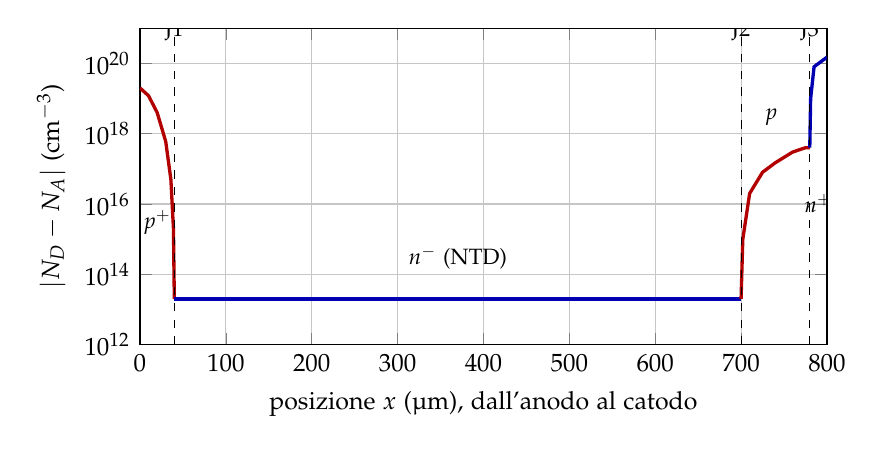
\begin{tikzpicture}
\begin{axis}[
  width=0.85\textwidth, height=5.6cm,
  xlabel={posizione $x$ (\unit{\um}), dall'anodo al catodo},
  ylabel={$|N_D-N_A|$ (\unit{\per\cm\cubed})},
  ymode=log, ymin=1e12, ymax=1e21,
  xmin=0, xmax=800,
  grid=both, minor grid style={gray!20}, major grid style={gray!45},
  font=\small, ytick={1e12,1e14,1e16,1e18,1e20},
]
% p+ emettitore di anodo: 0-40 um, profilo diffuso
\addplot[red!70!black,very thick] coordinates {(0,2e19) (10,1.2e19) (20,4e18) (30,6e17) (36,5e16) (39,2e15) (40,2e13)};
% base n-: 40-700 um
\addplot[blue!70!black,very thick] coordinates {(40,2e13) (700,2e13)};
% base p: 700-760 um, profilo gaussiano
\addplot[red!70!black,very thick] coordinates {(700,2e13) (702,1e15) (710,2e16) (725,8e16) (740,1.5e17) (760,3e17) (775,4e17) (780,4e17)};
% n+ catodo: 780-800
\addplot[blue!70!black,very thick] coordinates {(780,4e17) (781,1e19) (785,8e19) (800,1.5e20)};
% giunzioni
\draw[dashed] (axis cs:40,1e12) -- (axis cs:40,1e21) node[above,pos=0.93,font=\footnotesize] {J1};
\draw[dashed] (axis cs:700,1e12) -- (axis cs:700,1e21) node[above,pos=0.93,font=\footnotesize] {J2};
\draw[dashed] (axis cs:780,1e12) -- (axis cs:780,1e21) node[above,pos=0.93,font=\footnotesize] {J3};
\node[font=\footnotesize] at (axis cs:20,3e15) {$p^+$};
\node[font=\footnotesize] at (axis cs:370,3e14) {$n^-$ (NTD)};
\node[font=\footnotesize] at (axis cs:735,3e18) {$p$};
\node[font=\footnotesize] at (axis cs:790,1e16) {$n^+$};
\end{axis}
\end{tikzpicture}
\caption{Profilo di drogaggio netto tipico di un tiristore da \qty{4.5}{\kV} (valori indicativi). Gli emettitori sono diffusi con profilo gaussiano/erfc; la base $n^-$ è il substrato NTD uniforme.}
\label{fig:doping}
\end{figure}

\subsection{Diagramma a bande all'equilibrio}
All'equilibrio termodinamico (nessuna tensione applicata) il livello di Fermi $E_F$ è costante lungo tutto il dispositivo e le bande si piegano in corrispondenza delle tre giunzioni (Fig.~\ref{fig:bande}). Ogni giunzione presenta un potenziale di \en{built-in}
\begin{equation}
  V_{bi} = \frac{kT}{q}\ln\frac{N_A N_D}{n_i^2},
  \label{eq:vbi}
\end{equation}
che vale circa \qty{0.75}{\V} per J1 ($p^+/n^-$), \qty{0.65}{\V} per J2 ($n^-/p$) e \qty{0.9}{\V} per J3 ($p/n^+$) a \qty{300}{\K}. Le barriere di J1 e J3 si oppongono all'iniezione degli emettitori; J2 è orientata in senso opposto. Il risultato è un profilo di bande ``a doppia gobba'': gli elettroni del catodo vedono una barriera per entrare nella base p, le lacune dell'anodo vedono una barriera per entrare nella base n. Tutto il funzionamento del tiristore consiste nel modulare queste barriere: abbassarle (conduzione) o alzarne una (J2 in blocco diretto, J1 in blocco inverso).

\begin{figure}[htbp]
\centering
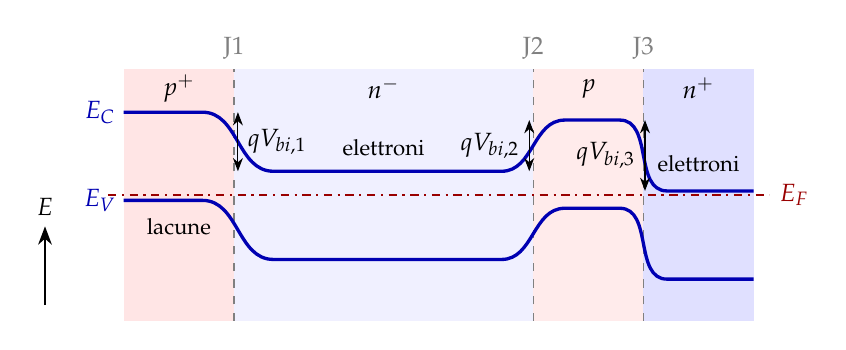
\begin{tikzpicture}[x=1cm,y=1cm,font=\small]
  % regioni
  \fill[red!10]  (0,-1.6) rectangle (1.4,1.6);
  \fill[blue!6]  (1.4,-1.6) rectangle (5.2,1.6);
  \fill[red!8]   (5.2,-1.6) rectangle (6.6,1.6);
  \fill[blue!12] (6.6,-1.6) rectangle (8,1.6);
  \node at (0.7,1.35) {$p^+$};
  \node at (3.3,1.35) {$n^-$};
  \node at (5.9,1.35) {$p$};
  \node at (7.3,1.35) {$n^+$};
  \draw[dashed,gray] (1.4,-1.6) -- (1.4,1.6) node[above] {J1};
  \draw[dashed,gray] (5.2,-1.6) -- (5.2,1.6) node[above] {J2};
  \draw[dashed,gray] (6.6,-1.6) -- (6.6,1.6) node[above] {J3};
  % Fermi level
  \draw[thick,red!60!black,dash dot] (-0.2,0) -- (8.2,0) node[right] {$E_F$};
  % E_C
  \draw[very thick,blue!70!black]
    (0,1.05) -- (1.0,1.05) to[out=0,in=180] (1.9,0.30) -- (4.8,0.30)
    to[out=0,in=180] (5.6,0.95) -- (6.3,0.95) to[out=0,in=180] (6.9,0.05) -- (8,0.05);
  \node[blue!70!black] at (-0.3,1.05) {$E_C$};
  % E_V
  \draw[very thick,blue!70!black]
    (0,-0.07) -- (1.0,-0.07) to[out=0,in=180] (1.9,-0.82) -- (4.8,-0.82)
    to[out=0,in=180] (5.6,-0.17) -- (6.3,-0.17) to[out=0,in=180] (6.9,-1.07) -- (8,-1.07);
  \node[blue!70!black] at (-0.3,-0.07) {$E_V$};
  % barriere
  \draw[dim] (1.45,0.30) -- (1.45,1.05) node[midway,right] {$qV_{bi,1}$};
  \draw[dim] (5.15,0.30) -- (5.15,0.95) node[midway,left] {$qV_{bi,2}$};
  \draw[dim] (6.62,0.05) -- (6.62,0.95) node[midway,left] {$qV_{bi,3}$};
  % portatori
  \node[font=\footnotesize] at (0.7,-0.4) {lacune};
  \node[font=\footnotesize] at (3.3,0.6) {elettroni};
  \node[font=\footnotesize] at (7.3,0.4) {elettroni};
  \draw[ax] (-1.0,-1.4) -- (-1.0,-0.4) node[above] {$E$};
\end{tikzpicture}
\caption{Diagramma a bande qualitativo del tiristore all'equilibrio: $E_F$ costante, tre barriere di potenziale. In blocco diretto la barriera di J2 si alza di $q\VAK$; in conduzione tutte e tre le giunzioni sono polarizzate direttamente e le barriere si abbassano.}
\label{fig:bande}
\end{figure}

\subsection{Realizzazione fisica}
Nei dispositivi di grande area il chip è un intero \en{wafer} di silicio (diametro \qtyrange{50}{150}{\mm}) montato fra due dischi di molibdeno o tungsteno che compensano la dilatazione termica; il contenitore ceramico a pressione (\en{press-pack}, \en{hockey-puck}) garantisce il contatto elettrico e termico su entrambe le facce. Il gate è portato all'esterno da una molla o da un contatto centrale. La struttura di catodo non è un semplice strato $n^+$ continuo ma un disegno interdigitato di emettitori $n^+$, \en{shorts} e strutture di gate distribuite (\S\ref{sec:spreading}) che determina in modo decisivo le prestazioni dinamiche.

% =====================================================================
\section{Il modello a due transistori}
% =====================================================================
\label{sec:2T}
La chiave interpretativa del tiristore è osservare che la struttura $p^+ n^- p\, n^+$ contiene due transistori bipolari che condividono le regioni centrali (Fig.~\ref{fig:2T}): un p-n-p ($p^+ n^- p$: emettitore = anodo, base = N1, collettore = P2) e un n-p-n ($n^- p\, n^+$: emettitore = catodo, base = P2, collettore = N1). Il collettore di ciascuno è la base dell'altro: la giunzione J2 è il collettore comune.

\begin{figure}[htbp]
\centering
\begin{subfigure}[b]{0.22\textwidth}
\centering
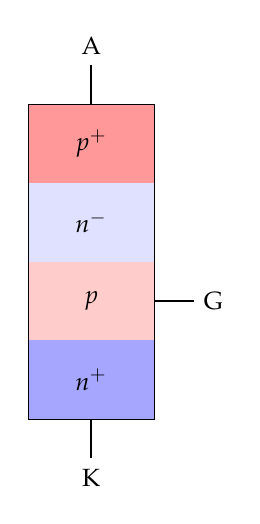
\begin{tikzpicture}[x=1cm,y=1cm,font=\small]
  \fill[layerPp] (0,3) rectangle (1.6,4); \node at (0.8,3.5) {$p^+$};
  \fill[layerN]  (0,2) rectangle (1.6,3); \node at (0.8,2.5) {$n^-$};
  \fill[layerP]  (0,1) rectangle (1.6,2); \node at (0.8,1.5) {$p$};
  \fill[layerNp] (0,0) rectangle (1.6,1); \node at (0.8,0.5) {$n^+$};
  \draw (0,0) rectangle (1.6,4);
  \draw[thick] (0.8,4) -- (0.8,4.5) node[above] {A};
  \draw[thick] (0.8,0) -- (0.8,-0.5) node[below] {K};
  \draw[thick] (1.6,1.5) -- (2.1,1.5) node[right] {G};
\end{tikzpicture}
\caption{struttura}
\end{subfigure}
\hfill
\begin{subfigure}[b]{0.36\textwidth}
\centering
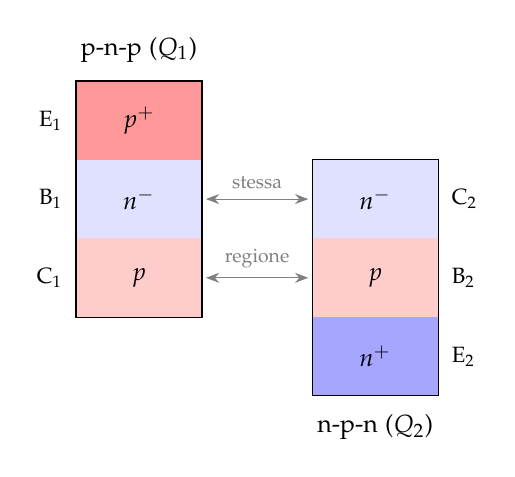
\begin{tikzpicture}[x=1cm,y=1cm,font=\small]
  % pnp a sinistra (alto), npn a destra (basso), sovrapposti sulle regioni centrali
  \fill[layerPp] (0,3) rectangle (1.6,4); \node at (0.8,3.5) {$p^+$};
  \fill[layerN]  (0,2) rectangle (1.6,3); \node at (0.8,2.5) {$n^-$};
  \fill[layerP]  (0,1) rectangle (1.6,2); \node at (0.8,1.5) {$p$};
  \draw (0,1) rectangle (1.6,4);
  \node[left,font=\footnotesize] at (-0.05,3.5) {E$_1$};
  \node[left,font=\footnotesize] at (-0.05,2.5) {B$_1$};
  \node[left,font=\footnotesize] at (-0.05,1.5) {C$_1$};
  \node at (0.8,4.4) {p-n-p ($Q_1$)};
  \fill[layerN]  (3.0,2) rectangle (4.6,3); \node at (3.8,2.5) {$n^-$};
  \fill[layerP]  (3.0,1) rectangle (4.6,2); \node at (3.8,1.5) {$p$};
  \fill[layerNp] (3.0,0) rectangle (4.6,1); \node at (3.8,0.5) {$n^+$};
  \draw (3.0,0) rectangle (4.6,3);
  \node[right,font=\footnotesize] at (4.65,2.5) {C$_2$};
  \node[right,font=\footnotesize] at (4.65,1.5) {B$_2$};
  \node[right,font=\footnotesize] at (4.65,0.5) {E$_2$};
  \node at (3.8,-0.4) {n-p-n ($Q_2$)};
  \draw[<->,>=Stealth,gray] (1.65,2.5) -- (2.95,2.5) node[midway,above,font=\scriptsize] {stessa};
  \draw[<->,>=Stealth,gray] (1.65,1.5) -- (2.95,1.5) node[midway,above,font=\scriptsize] {regione};
\end{tikzpicture}
\caption{separazione in due transistori}
\end{subfigure}
\hfill
\begin{subfigure}[b]{0.36\textwidth}
\centering
\begin{circuitikz}[scale=0.95,font=\small]
  \node[pnp,xscale=-1] (Q1) at (0,2.2) {};
  \node[npn] (Q2) at (2.4,0) {};
  \node[left] at (Q1.E) {};
  \node[font=\footnotesize] at (-0.55,2.2) {$Q_1$};
  \node[font=\footnotesize] at (2.95,0) {$Q_2$};
  \draw (Q1.E) -- (0,3.4) node[above] {A};
  \draw[->,>=Stealth] (0,3.35) -- (0,3.0) node[midway,right] {$\IA$};
  \draw (Q1.C) |- (Q2.B);
  \draw (Q2.C) |- (Q1.B);
  \draw (Q2.E) -- (2.4,-1.4) node[below] {K};
  \draw[->,>=Stealth] (2.4,-0.9) -- (2.4,-1.3) node[midway,right] {$\IK$};
  \draw (1.0,0) -- (1.0,-1.4) node[below] {G};
  \draw[->,>=Stealth] (1.0,-1.3) -- (1.0,-0.6) node[midway,left] {$\IG$};
  \fill (1.0,0) circle (1.2pt);
  \node[font=\footnotesize,right] at (0.0,0.85) {$I_{C1}=\alpha_1 \IA$};
  \node[font=\footnotesize,left] at (2.4,1.5) {$I_{C2}=\alpha_2 \IK$};
\end{circuitikz}
\caption{circuito equivalente}
\end{subfigure}
\caption{Modello a due transistori: la struttura p-n-p-n è scomposta in un p-n-p e un n-p-n con collettore comune (J2); ognuno alimenta la base dell'altro.}
\label{fig:2T}
\end{figure}

\subsection{Equazione di anodo}
Con $\alpha_1$ e $\alpha_2$ i guadagni di corrente a base comune dei due transistori e $I_{CO1}$, $I_{CO2}$ le correnti di saturazione inversa del collettore comune (entrambe corrente di leakage di J2), le correnti di collettore sono
\begin{equation}
  I_{C1} = \alpha_1 \IA + I_{CO1}, \qquad I_{C2} = \alpha_2 \IK + I_{CO2}.
\end{equation}
La corrente totale che attraversa J2 è la somma dei due collettori ed è uguale alla corrente di anodo, $\IA = I_{C1}+I_{C2}$, mentre al catodo $\IK = \IA + \IG$. Risolvendo:
\begin{equation}
  \boxed{\;\IA = \frac{\alpha_2 \IG + I_{CO1} + I_{CO2}}{1 - (\alpha_1 + \alpha_2)}\;}
  \label{eq:anodo}
\end{equation}
Questa equazione contiene tutta la fenomenologia del tiristore:
\begin{itemize}
  \item finché $\alpha_1+\alpha_2 \ll 1$, la corrente di anodo è la corrente di leakage di J2 leggermente amplificata: \textbf{blocco diretto};
  \item se $\alpha_1+\alpha_2 \to 1$ il denominatore si annulla e $\IA$ è limitata solo dal circuito esterno: \textbf{conduzione}. Il gate, che compare solo al numeratore, non ha più alcun effetto;
  \item l'innesco richiede di far crescere $\alpha_1+\alpha_2$ fino a uno; poiché i guadagni crescono con la corrente (\S\ref{sec:alpha}), \emph{qualunque} meccanismo che aumenti transitoriamente la corrente attraverso J2 (gate, $\dvdt$, valanga, temperatura, luce) può innescare il dispositivo.
\end{itemize}

Il modello va inteso come modello a piccoli segnali attorno a un punto di lavoro: in conduzione i due transistori sono in saturazione profonda, con entrambe le basi allagate da plasma, e i guadagni perdono il loro significato di parametri costanti. L'equazione~\eqref{eq:anodo} descrive però correttamente il confine fra blocco e conduzione.

\subsection{Dipendenza dei guadagni dalla corrente}
\label{sec:alpha}
Il guadagno a base comune è il prodotto dell'efficienza di emettitore $\gamma$ e del fattore di trasporto in base $\alpha_T$:
\begin{equation}
  \alpha = \gamma\,\alpha_T, \qquad
  \gamma = \frac{I_{E,\text{iniettata}}}{I_E}, \qquad
  \alpha_T = \frac{1}{\cosh(W_B/L_B)} \approx 1 - \frac{W_B^2}{2L_B^2},
  \label{eq:alpha}
\end{equation}
dove $W_B$ è lo spessore della base neutra e $L_B=\sqrt{D\tau}$ la lunghezza di diffusione dei minoritari in base. I due transistori sono molto diversi:
\begin{itemize}
  \item il p-n-p $Q_1$ ha la base $n^-$ larghissima ($W_N$ di centinaia di \unit{\um}, confrontabile o maggiore di $L_p$), quindi $\alpha_1$ è piccolo, dell'ordine di \numrange{0.2}{0.5}, e cresce con la tensione perché la regione di svuotamento di J2 riduce la base neutra effettiva (effetto Early);
  \item l'n-p-n $Q_2$ ha la base p sottile ($W_P\ll L_n$), quindi potenzialmente $\alpha_2$ è vicino a uno. È però proprio $\alpha_2$ che va tenuto basso a bassa corrente perché il dispositivo blocchi.
\end{itemize}
A basse densità di corrente $\gamma$ è piccolo per entrambi, perché la corrente di ricombinazione nella regione di svuotamento dell'emettitore (termine Sah--Noyce--Shockley, proporzionale a $e^{qV/2kT}$) domina sulla corrente di diffusione utile (proporzionale a $e^{qV/kT}$). Al crescere della corrente il termine di diffusione prevale e $\gamma\to1$. Inoltre in $Q_2$ i \en{cathode shorts} (\S\ref{sec:dvdt}) deviano a catodo la corrente di base finché la caduta laterale nella base p non raggiunge \qtyrange{0.6}{0.7}{\V}: sotto questa soglia J3 praticamente non inietta e $\alpha_2\approx0$. Il risultato complessivo è mostrato in Fig.~\ref{fig:alpha}: la somma $\alpha_1+\alpha_2$ è molto minore di uno alla corrente di leakage e raggiunge uno a una corrente dell'ordine della \en{latching current}. Ad alta corrente i guadagni tornano a diminuire per gli effetti di alta iniezione (caduta di $\gamma$ per \en{emitter push-out} e ricombinazione Auger), ma a quel punto il dispositivo è già in conduzione.

\begin{figure}[htbp]
\centering
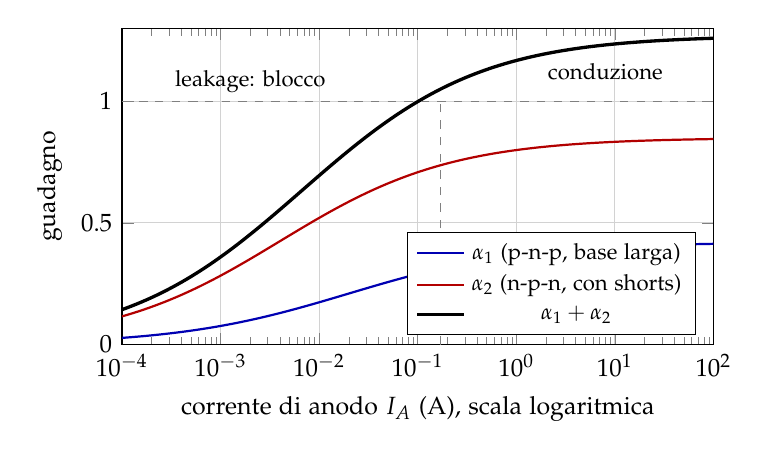
\begin{tikzpicture}
\begin{axis}[
  width=0.75\textwidth, height=5.6cm,
  xmode=log, xmin=1e-4, xmax=1e2,
  ymin=0, ymax=1.3,
  xlabel={corrente di anodo $\IA$ (A), scala logaritmica},
  ylabel={guadagno},
  grid=major, major grid style={gray!35},
  font=\small, legend pos=south east, legend style={font=\footnotesize},
  samples=120, domain=1e-4:1e2,
]
\addplot[blue!70!black,thick] {0.42*sqrt(x)/(sqrt(x)+sqrt(0.02))};
\addlegendentry{$\alpha_1$ (p-n-p, base larga)}
\addplot[red!70!black,thick] {0.85*sqrt(x)/(sqrt(x)+sqrt(0.004))};
\addlegendentry{$\alpha_2$ (n-p-n, con shorts)}
\addplot[black,very thick] {0.42*sqrt(x)/(sqrt(x)+sqrt(0.02))+0.85*sqrt(x)/(sqrt(x)+sqrt(0.004))};
\addlegendentry{$\alpha_1+\alpha_2$}
\addplot[gray,dashed,domain=1e-4:1e2] {1};
\draw[dashed,gray] (axis cs:0.17,0) -- (axis cs:0.17,1) node[pos=0.25,right,font=\footnotesize] {$\IA\approx\IL$};
\node[font=\footnotesize] at (axis cs:2e-3,1.08) {leakage: blocco};
\node[font=\footnotesize] at (axis cs:8,1.12) {conduzione};
\end{axis}
\end{tikzpicture}
\caption{Andamento qualitativo dei guadagni a base comune in funzione della corrente. Il blocco diretto è possibile perché $\alpha_1+\alpha_2\ll1$ alle correnti di leakage; l'innesco corrisponde al raggiungimento di $\alpha_1+\alpha_2=1$.}
\label{fig:alpha}
\end{figure}

% =====================================================================
\section{Stati di blocco}
% =====================================================================
\subsection{Blocco diretto}
Con $\VAK>0$ e gate aperto, J1 e J3 sono polarizzate direttamente (con pochi decimi di volt) e J2 è polarizzata inversamente e sostiene praticamente tutta la tensione. Poiché la base p è drogata \numrange{1e3}{1e4} volte più della base $n^-$, la regione di svuotamento di J2 si estende quasi interamente nella base $n^-$ (Fig.~\ref{fig:campo}a). Con l'approssimazione di svuotamento brusco (giunzione unilaterale):
\begin{equation}
  W_D(V) = \sqrt{\frac{2\varepsilon_{Si} V}{q N_D}}, \qquad
  E_{max} = \sqrt{\frac{2 q N_D V}{\varepsilon_{Si}}} = \frac{2V}{W_D}.
  \label{eq:WD}
\end{equation}
Per $N_D=\qty{1e13}{\per\cm\cubed}$ e $V=\qty{6.5}{\kV}$ si ottiene $W_D\approx\qty{920}{\um}$ e $E_{max}\approx\qty{1.4e5}{\V\per\cm}$, vicino al campo critico di rottura del silicio a quel drogaggio ($E_c\approx\qty{1.7e5}{\V\per\cm}$). La tensione di rottura a valanga della giunzione piana $n^-/p$ vale, con la formula di Baliga~\cite{baliga},
\begin{equation}
  BV_{pp} \approx \num{5.34e13}\, N_D^{-3/4} \;\text{[V, $N_D$ in \unit{\per\cm\cubed}]},
\end{equation}
cioè circa \qty{9.5}{\kV} per $N_D=\qty{1e13}{\per\cm\cubed}$: il dispositivo da \qty{6.5}{\kV} lavora con un margine del \qty{30}{\percent} circa, necessario per la terminazione di bordo (\en{bevel}) e per il meccanismo di \en{breakover} descritto sotto.

\begin{figure}[htbp]
\centering
\begin{subfigure}[b]{0.48\textwidth}
\centering
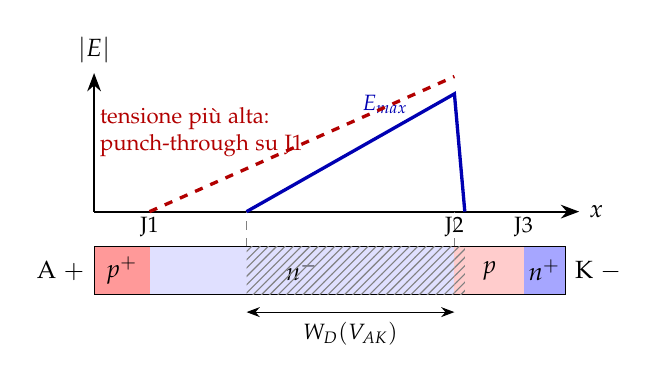
\begin{tikzpicture}[x=0.88cm,y=0.88cm,font=\small]
  \fill[layerPp] (0,0) rectangle (0.8,0.7);
  \fill[layerN]  (0.8,0) rectangle (5.2,0.7);
  \fill[layerP]  (5.2,0) rectangle (6.2,0.7);
  \fill[layerNp] (6.2,0) rectangle (6.8,0.7);
  \draw (0,0) rectangle (6.8,0.7);
  \node at (0.4,0.35) {$p^+$}; \node at (3,0.35) {$n^-$}; \node at (5.7,0.35) {$p$}; \node at (6.5,0.35) {$n^+$};
  \node[above,font=\footnotesize] at (0.8,0.7) {J1}; \node[above,font=\footnotesize] at (5.2,0.7) {J2}; \node[above,font=\footnotesize] at (6.2,0.7) {J3};
  \node[left] at (0,0.35) {A $+$}; \node[right] at (6.8,0.35) {K $-$};
  % svuotamento
  \fill[pattern=north east lines,pattern color=gray] (2.2,0) rectangle (5.2,0.7);
  \fill[pattern=north east lines,pattern color=gray] (5.2,0) rectangle (5.35,0.7);
  \draw[dim] (2.2,-0.25) -- (5.2,-0.25) node[midway,below,font=\footnotesize] {$W_D(\VAK)$};
  % campo
  \draw[ax] (0,1.2) -- (7,1.2) node[right] {$x$};
  \draw[ax] (0,1.2) -- (0,3.2) node[above] {$|E|$};
  \draw[very thick,blue!70!black] (2.2,1.2) -- (5.2,2.9) -- (5.35,1.2);
  \node[blue!70!black,font=\footnotesize] at (4.2,2.75) {$E_{max}$};
  \draw[very thick,red!70!black,dashed] (0.8,1.2) -- (5.2,3.15);
  \node[red!70!black,font=\footnotesize,align=left] at (1.55,2.35) {tensione più alta:\\ punch-through su J1};
  \draw[dashed,gray] (2.2,0.7) -- (2.2,1.2);
  \draw[dashed,gray] (5.2,0.7) -- (5.2,1.2);
\end{tikzpicture}
\caption{blocco diretto: J2 sostiene la tensione}
\end{subfigure}
\hfill
\begin{subfigure}[b]{0.48\textwidth}
\centering
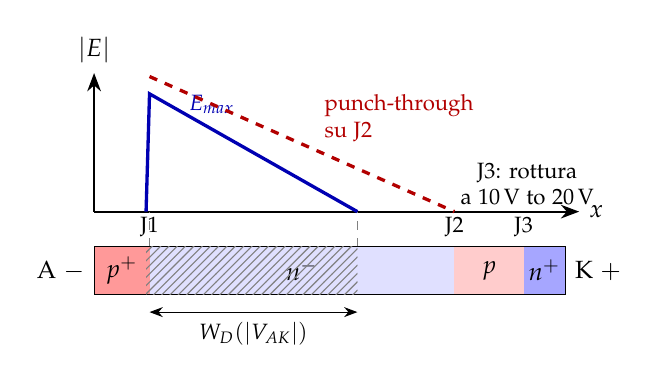
\begin{tikzpicture}[x=0.88cm,y=0.88cm,font=\small]
  \fill[layerPp] (0,0) rectangle (0.8,0.7);
  \fill[layerN]  (0.8,0) rectangle (5.2,0.7);
  \fill[layerP]  (5.2,0) rectangle (6.2,0.7);
  \fill[layerNp] (6.2,0) rectangle (6.8,0.7);
  \draw (0,0) rectangle (6.8,0.7);
  \node at (0.4,0.35) {$p^+$}; \node at (3,0.35) {$n^-$}; \node at (5.7,0.35) {$p$}; \node at (6.5,0.35) {$n^+$};
  \node[above,font=\footnotesize] at (0.8,0.7) {J1}; \node[above,font=\footnotesize] at (5.2,0.7) {J2}; \node[above,font=\footnotesize] at (6.2,0.7) {J3};
  \node[left] at (0,0.35) {A $-$}; \node[right] at (6.8,0.35) {K $+$};
  \fill[pattern=north east lines,pattern color=gray] (0.8,0) rectangle (3.8,0.7);
  \fill[pattern=north east lines,pattern color=gray] (0.75,0) rectangle (0.8,0.7);
  \draw[dim] (0.8,-0.25) -- (3.8,-0.25) node[midway,below,font=\footnotesize] {$W_D(|\VAK|)$};
  \draw[ax] (0,1.2) -- (7,1.2) node[right] {$x$};
  \draw[ax] (0,1.2) -- (0,3.2) node[above] {$|E|$};
  \draw[very thick,blue!70!black] (0.75,1.2) -- (0.8,2.9) -- (3.8,1.2);
  \node[blue!70!black,font=\footnotesize] at (1.7,2.75) {$E_{max}$};
  \draw[very thick,red!70!black,dashed] (0.8,3.15) -- (5.2,1.2);
  \node[red!70!black,font=\footnotesize,align=left] at (4.4,2.55) {punch-through\\ su J2};
  % J3 piccola
  \node[font=\footnotesize,align=center] at (6.25,1.6) {J3: rottura\\ a \qtyrange{10}{20}{\V}};
  \draw[dashed,gray] (3.8,0.7) -- (3.8,1.2);
  \draw[dashed,gray] (0.8,0.7) -- (0.8,1.2);
\end{tikzpicture}
\caption{blocco inverso: J1 sostiene la tensione}
\end{subfigure}
\caption{Regione di svuotamento (tratteggio) e profilo del campo elettrico nei due stati di blocco. In entrambi i casi il campo si sviluppa nella base $n^-$, che deve essere abbastanza spessa da evitare che lo svuotamento raggiunga la giunzione opposta (\en{punch-through}).}
\label{fig:campo}
\end{figure}

\paragraph{Corrente di leakage.} La corrente in blocco diretto non è la sola corrente di generazione termica nella regione di svuotamento di J2,
\begin{equation}
  J_{gen} = \frac{q\,n_i\,W_D}{2\tau_g},
\end{equation}
ma questa corrente amplificata dal fattore $1/(1-\alpha_1-\alpha_2)$ dell'eq.~\eqref{eq:anodo}, perché le lacune generate in J2 entrano nella base p come corrente di base dell'n-p-n, e gli elettroni entrano nella base n come corrente di base del p-n-p. A parità di giunzione, un tiristore ha quindi leakage maggiore di un diodo con la stessa base $n^-$. La corrente di generazione raddoppia circa ogni \qty{8}{\K} ($n_i \propto T^{3/2}e^{-E_g/2kT}$), e contemporaneamente i guadagni crescono con la temperatura: per questo la tensione di blocco specificata ($\VDRM$) è garantita solo fino a $T_{j,max}$, tipicamente \qty{125}{\celsius}, oltre la quale il dispositivo può auto-innescarsi (\S\ref{sec:altri}).

\paragraph{Breakover.} Se la tensione diretta cresce, il campo in J2 raggiunge valori a cui si ha moltiplicazione a valanga con fattore $M(V)$, approssimabile empiricamente con $M = [1-(V/BV)^n]^{-1}$, $n\approx\numrange{4}{6}$. Le correnti dei due collettori sono moltiplicate per $M$ e la condizione di perdita del blocco diventa
\begin{equation}
  M(V)\,(\alpha_1+\alpha_2) = 1 \quad\Longrightarrow\quad
  \VBO = BV\,\bigl(1-\alpha_1-\alpha_2\bigr)^{1/n}.
  \label{eq:VBO}
\end{equation}
La tensione di \en{breakover} $\VBO$ è quindi sempre inferiore alla tensione di rottura di J2 isolata, e tanto più bassa quanto più alti sono i guadagni: è la versione a quattro strati della $BV_{CEO}<BV_{CBO}$ del transistor a base aperta. Nella pratica $\VDRM$ è specificata con margine rispetto a $\VBO$ e il funzionamento in \en{breakover} è ammesso solo in dispositivi progettati per questo (BOD, \en{break-over diode}, usati come protezione).

\subsection{Blocco inverso}
Con $\VAK<0$ le giunzioni J1 e J3 sono polarizzate inversamente e J2 direttamente (Fig.~\ref{fig:campo}b). J3 ($p/n^+$, con base p a $\sim\qty{e17}{\per\cm\cubed}$) ha una tensione di rottura di soli \qtyrange{10}{20}{\V} ed è in ogni caso cortocircuitata dai \en{cathode shorts}: è J1 ($p^+/n^-$) che sostiene la tensione inversa, e lo fa con la stessa base $n^-$ usata in blocco diretto. Nel tiristore simmetrico convenzionale $\VRRM\approx\VDRM$, e questa capacità di blocco inverso è ciò che permette di usarlo direttamente nei ponti a commutazione di rete senza diodi in serie.

Lo svuotamento inverso si estende da J1 verso J2 e, nel modello a due transistori, corrisponde a un p-n-p a base aperta: anche in inverso il guadagno $\alpha_1$ abbassa la tensione di rottura rispetto a quella della giunzione isolata, e il leakage inverso è di ordine simile a quello diretto.

\subsection{Punch-through e dimensionamento della base n}
In blocco diretto la regione di svuotamento non deve raggiungere J1 e in blocco inverso non deve raggiungere J2: in entrambi i casi l'emettitore/base raggiunto inietterebbe portatori direttamente nel campo, con perdita immediata del blocco (\en{punch-through}). Nei tiristori simmetrici (\en{non punch-through}, NPT) questo impone
\begin{equation}
  W_N > W_D(V_{max}) + \text{margine} \approx \sqrt{\frac{2\varepsilon_{Si} V_{max}}{qN_D}} + (\numrange{50}{100}\;\unit{\um}),
\end{equation}
da cui la base spessa e, in conduzione, la caduta diretta relativamente alta dei dispositivi ad alta tensione. Il tiristore asimmetrico (ASCR) introduce uno strato \en{buffer} $n$ tra base $n^-$ e emettitore di anodo (\en{field stop}): il campo può essere troncato e la base ridotta di circa il \qty{40}{\percent}, con vantaggi su $V_T$, $Q_{rr}$ e $\tq$, ma il blocco inverso si riduce a poche decine di volt. L'RCT (\en{reverse-conducting thyristor}) integra un diodo in antiparallelo sullo stesso chip.

\subsection{Terminazione di bordo}
Le formule precedenti valgono per la giunzione piana infinita. Al bordo del wafer il campo si concentra e ridurrebbe la tensione di rottura del \qtyrange{30}{50}{\percent}: nei tiristori di potenza si usa per questo la smussatura (\en{bevel}) del bordo, positiva o negativa a seconda della giunzione, che riduce il campo superficiale sotto quello di volume. È uno degli aspetti tecnologici più delicati e la ragione per cui i dispositivi di grande area sono passivati e incapsulati in ambiente controllato.

% =====================================================================
\section{Innesco}
% =====================================================================
\subsection{Innesco da gate}
Il gate è un contatto ohmico sulla base p. Iniettando una corrente $\IG$ (positiva entrante nel gate, con il gate positivo rispetto al catodo) si polarizza direttamente J3 nella zona adiacente al gate e l'emettitore $n^+$ inietta elettroni nella base p. In termini di transistori: $\IG$ è corrente di base di $Q_2$. La sequenza è la seguente (Fig.~\ref{fig:innesco}):
\begin{enumerate}
  \item gli elettroni iniettati da J3 attraversano la sottile base p per diffusione e vengono raccolti da J2 (polarizzata inversamente): corrente di collettore $\alpha_2 (\IG + \dots)$;
  \item questi elettroni entrano nella base $n^-$ e ne abbassano il potenziale: la corrente di collettore di $Q_2$ è corrente di base per $Q_1$;
  \item J1 si polarizza più direttamente e l'emettitore $p^+$ inietta lacune nella base $n^-$; quelle che attraversano la base larga arrivano a J2 e vengono raccolte nella base p: corrente di collettore $\alpha_1 \IA$;
  \item le lacune raccolte in P2 sono ulteriore corrente di base per $Q_2$, che si somma a $\IG$: l'anello è chiuso.
\end{enumerate}
Ogni giro dell'anello moltiplica la corrente per $\alpha_1\alpha_2/(1-\dots)$; con guadagni crescenti con la corrente si arriva rapidamente a $\alpha_1+\alpha_2=1$. A quel punto entrambe le basi si riempiono di portatori, J2 passa da polarizzazione inversa a diretta e la tensione ai capi del dispositivo crolla a \qtyrange{1}{2}{\V}. Dal punto di vista del gate, la corrente esterna può ora essere rimossa: la corrente di base di $Q_2$ è fornita interamente dal collettore di $Q_1$.

\begin{figure}[htbp]
\centering
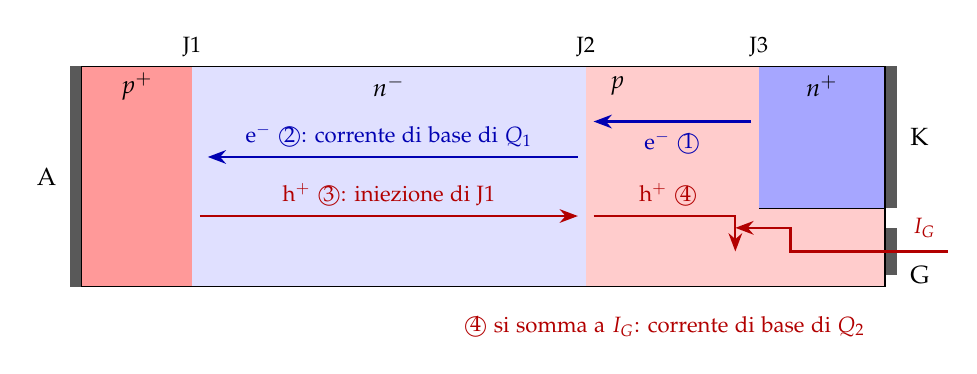
\begin{tikzpicture}[x=1cm,y=1cm,font=\small]
  \fill[layerPp] (0,0) rectangle (1.4,2.8);
  \fill[layerN]  (1.4,0) rectangle (6.4,2.8);
  \fill[layerP]  (6.4,0) rectangle (8.6,2.8);
  \fill[layerNp] (8.6,1.0) rectangle (10.2,2.8);
  \fill[layerP]  (8.6,0) rectangle (10.2,1.0);
  \fill[metal] (-0.15,0) rectangle (0,2.8);
  \fill[metal] (10.2,1.0) rectangle (10.35,2.8);
  \fill[metal] (10.2,0.15) rectangle (10.35,0.75);
  \draw (0,0) rectangle (10.2,2.8);
  \draw (8.6,1.0) -- (10.2,1.0);
  \node at (0.7,2.55) {$p^+$}; \node at (3.9,2.55) {$n^-$}; \node at (6.8,2.55) {$p$}; \node at (9.4,2.55) {$n^+$};
  \node[above,font=\footnotesize] at (1.4,2.8) {J1}; \node[above,font=\footnotesize] at (6.4,2.8) {J2}; \node[above,font=\footnotesize] at (8.6,2.8) {J3};
  \node[left] at (-0.2,1.4) {A};
  \node[right] at (10.4,1.9) {K};
  \node[right] at (10.4,0.15) {G};
  % gate current (holes) entering p base
  \draw[->,>=Stealth,thick,red!70!black] (11.0,0.45) -- (9.0,0.45) -- (9.0,0.75) -- (8.3,0.75);
  \node[red!70!black,font=\footnotesize,above] at (10.7,0.5) {$\IG$};
  % (1) electrons from n+ into p, to J2
  \draw[->,>=Stealth,thick,blue!70!black] (8.5,2.1) -- (6.5,2.1);
  \node[blue!70!black,font=\footnotesize,below] at (7.5,2.1) {e$^-$ \textcircled{1}};
  % (2) electrons into n base (base current of Q1)
  \draw[->,>=Stealth,thick,blue!70!black] (6.3,1.65) -- (1.6,1.65);
  \node[blue!70!black,font=\footnotesize,above] at (3.9,1.65) {e$^-$ \textcircled{2}: corrente di base di $Q_1$};
  % (3) holes from p+ into n-
  \draw[->,>=Stealth,thick,red!70!black] (1.5,0.9) -- (6.3,0.9);
  \node[red!70!black,font=\footnotesize,above] at (3.9,0.9) {h$^+$ \textcircled{3}: iniezione di J1};
  % (4) holes collected into p base
  \draw[->,>=Stealth,thick,red!70!black] (6.5,0.9) -- (8.3,0.9) -- (8.3,0.45);
  \node[red!70!black,font=\footnotesize,above] at (7.45,0.9) {h$^+$ \textcircled{4}};
  \node[font=\footnotesize,align=center,red!70!black] at (7.4,-0.5) {\textcircled{4} si somma a $\IG$: corrente di base di $Q_2$};
\end{tikzpicture}
\caption{Sequenza di innesco: la corrente di gate fa iniettare J3; gli elettroni raccolti da J2 pilotano l'emettitore di anodo, le cui lacune ritornano nella base p come corrente di base aggiuntiva. La retroazione è positiva.}
\label{fig:innesco}
\end{figure}

I \en{data sheet} specificano la corrente e la tensione di gate di innesco garantite ($I_{GT}$, $V_{GT}$: per un dispositivo di grande area \qtyrange{100}{400}{\mA} e \qtyrange{1.5}{3}{\V} a \qty{25}{\celsius}) e i valori massimi sotto i quali l'innesco è garantito \emph{non} avvenire ($I_{GD}$, $V_{GD}$, importanti per l'immunità al rumore). $I_{GT}$ diminuisce con la temperatura e aumenta a bassa temperatura (a \qty{-40}{\celsius} può raddoppiare). Nella pratica il gate viene pilotato con un impulso molto più forte del minimo (\en{hard gate drive}: alcuni ampere con fronte di salita di \qty{1}{\A\per\us} o più, seguiti da una corrente di mantenimento, \en{back-porch}) per ridurre il tempo di ritardo, aumentare l'area inizialmente accesa e quindi la capacità di $\didt$ (\S\ref{sec:spreading}).

\subsection{Latching current e holding current}
Perché l'innesco sia completo, la corrente di anodo deve superare, prima che l'impulso di gate finisca, la \en{latching current} $\IL$: il valore minimo di $\IA$ a cui $\alpha_1+\alpha_2=1$ senza il contributo del gate. Una volta acceso, il dispositivo resta in conduzione finché $\IA$ non scende sotto la \en{holding current} $\IH$, con $\IH<\IL$ (tipicamente $\IL\approx\numrange{2}{3}\,\IH$). La differenza dipende dalla geometria: durante l'innesco conduce solo l'area vicina al gate, e la densità di corrente necessaria a sostenere la rigenerazione va raggiunta in quella piccola area; in conduzione stabilizzata l'intera area è attiva e la corrente totale necessaria per la stessa densità è minore. Entrambi i parametri diminuiscono con la temperatura (i guadagni aumentano) e aumentano con la densità di \en{cathode shorts}. Valori tipici per un dispositivo di grande area: $\IH\approx\qtyrange{100}{400}{\mA}$, $\IL\approx\qtyrange{0.3}{1}{\A}$.

\subsection{Innesco per \texorpdfstring{$\dvdt$}{dv/dt} e \en{cathode shorts}}
\label{sec:dvdt}
La giunzione J2 in blocco ha una capacità di svuotamento
\begin{equation}
  C_{J2}(V) = \frac{\varepsilon_{Si} A}{W_D(V)} \propto V^{-1/2},
\end{equation}
molto grande in un dispositivo di grande area (nF a bassa tensione). Una rapida crescita della tensione diretta produce una corrente di spostamento
\begin{equation}
  i_{J2} = C_{J2}\,\frac{\dd v}{\dd t}
\end{equation}
che, esattamente come la corrente di gate, è corrente di base per entrambi i transistori: le lacune attraversano la base p verso il catodo, gli elettroni la base n verso l'anodo. Se $i_{J2}$ è sufficiente a portare $\alpha_1+\alpha_2$ a uno, il tiristore si innesca senza comando (\en{dv/dt turn-on}). Questo è indesiderato (accensione fuori fase, perdita del controllo, sollecitazione localizzata perché l'innesco è disomogeneo) e i \en{data sheet} specificano il valore critico ($\dvdt$)$_{cr}$, tipicamente \qtyrange{500}{2000}{\V\per\us}, misurato con una rampa esponenziale fino a $\VDRM$ a $T_{j,max}$.

Il rimedio strutturale sono i \en{cathode shorts} (Fig.~\ref{fig:shorts}): la metallizzazione di catodo contatta, oltre all'emettitore $n^+$, anche la base p attraverso una griglia di piccole aperture nell'emettitore. La corrente di lacune che attraversa la base p scorre lateralmente verso lo \en{short} più vicino attraverso la resistenza distribuita $R_p$ della base p. Finché la caduta $i\,R_p$ resta sotto la tensione di soglia di J3 ($\approx\qty{0.6}{\V}$), l'emettitore $n^+$ non inietta: $\alpha_2\approx0$ e il dispositivo non si innesca. Il gate reale funziona sullo stesso principio, ma inietta la corrente nel punto della base p più lontano dagli \en{shorts}. Gli \en{shorts} aumentano l'immunità al $\dvdt$ e alla temperatura, ma a prezzo di una maggiore corrente di gate, di $\IH$ e $\IL$ più alte e di una minore capacità di $\didt$ (perdita di area di emettitore). La densità e la geometria degli \en{shorts} sono un parametro di progetto centrale del dispositivo.

\begin{figure}[htbp]
\centering
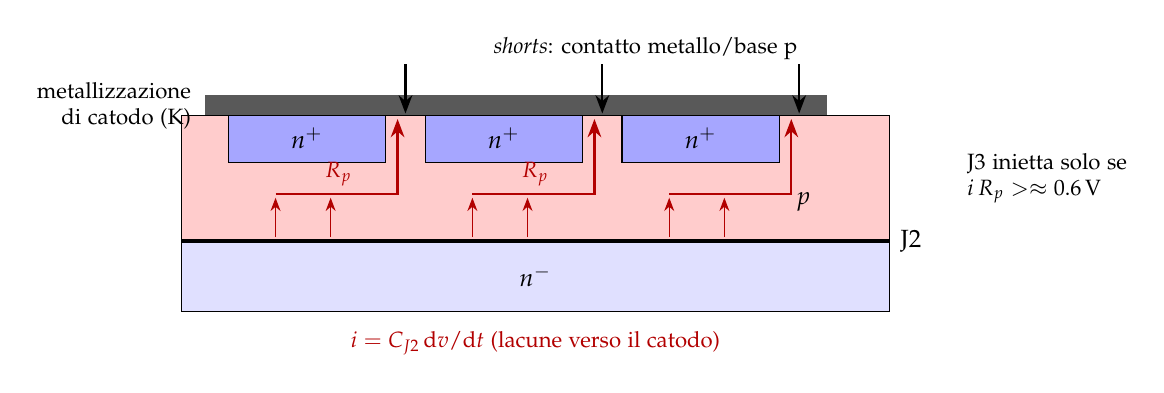
\begin{tikzpicture}[x=1cm,y=1cm,font=\small]
  % p base
  \fill[layerP] (0,0) rectangle (9,1.6);
  \fill[layerN] (0,-0.9) rectangle (9,0);
  % n+ emitter islands
  \foreach \x in {0.6,3.1,5.6} {
    \fill[layerNp] (\x,1.0) rectangle (\x+2.0,1.6);
    \draw (\x,1.0) rectangle (\x+2.0,1.6);
    \node at (\x+1.0,1.3) {$n^+$};
  }
  % cathode metal continuous on top
  \fill[metal] (0.3,1.6) rectangle (8.2,1.85);
  \node[left,font=\footnotesize,align=right] at (0.25,1.72) {metallizzazione\\ di catodo (K)};
  % shorts markers
  \foreach \x in {2.85,5.35,7.85} {
    \draw[<-,>=Stealth,thick] (\x,1.62) -- (\x,2.25);
  }
  \node[font=\footnotesize] at (5.9,2.45) {\en{shorts}: contatto metallo/base p};
  \node at (7.9,0.5) {$p$};
  \node at (4.5,-0.45) {$n^-$};
  \draw (0,-0.9) rectangle (9,1.6);
  \draw[junc] (0,0) -- (9,0) node[right] {J2};
  % displacement current: holes from J2 up into p base, laterally to shorts
  \foreach \x in {1.2,1.9,3.7,4.4,6.2,6.9} {
    \draw[->,>=Stealth,red!70!black] (\x,0.05) -- (\x,0.55);
  }
  \draw[->,>=Stealth,thick,red!70!black] (1.2,0.6) -- (2.75,0.6) -- (2.75,1.55);
  \draw[->,>=Stealth,thick,red!70!black] (3.7,0.6) -- (5.25,0.6) -- (5.25,1.55);
  \draw[->,>=Stealth,thick,red!70!black] (6.2,0.6) -- (7.75,0.6) -- (7.75,1.55);
  \node[red!70!black,font=\footnotesize] at (2.0,0.85) {$R_p$};
  \node[red!70!black,font=\footnotesize] at (4.5,0.85) {$R_p$};
  \node[red!70!black,font=\footnotesize,align=center] at (4.5,-1.3) {$i = C_{J2}\,\dvdt$ (lacune verso il catodo)};
  \node[font=\footnotesize,align=left] at (11.0,0.8) {J3 inietta solo se\\ $i\,R_p > \approx\qty{0.6}{\V}$};
\end{tikzpicture}
\caption{Struttura a \en{cathode shorts}: la corrente capacitiva di J2 viene deviata a catodo attraverso la base p senza polarizzare l'emettitore $n^+$, finché la caduta laterale non supera la soglia di J3.}
\label{fig:shorts}
\end{figure}

A livello di circuito, il $\dvdt$ è limitato dallo \en{snubber} RC in parallelo al dispositivo, dimensionato anche per contenere la sovratensione al \en{reverse recovery} (\S\ref{sec:rr}); l'induttanza di rete o di commutazione contribuisce a limitare il $\dvdt$ alla riapplicazione della tensione.

\subsection{Altri meccanismi di innesco}
\label{sec:altri}
Tutto ciò che aumenta la corrente attraverso J2 può chiudere l'anello:
\begin{itemize}
  \item \textbf{Tensione} (\en{breakover}): moltiplicazione a valanga in J2, eq.~\eqref{eq:VBO}. L'innesco parte dal punto di campo massimo (spesso al bordo o in un difetto) e non dall'area di gate: è disomogeneo e potenzialmente distruttivo per $\didt$ elevati.
  \item \textbf{Temperatura}: il leakage cresce esponenzialmente con $T_j$ e i guadagni con esso; oltre $T_{j,max}$ un tiristore in blocco a $\VDRM$ può auto-innescarsi. Esiste anche un meccanismo di \en{thermal runaway}: le perdite di leakage a tensione elevata scaldano la giunzione, che aumenta il leakage.
  \item \textbf{Luce} (LTT, \en{light-triggered thyristor}): una fibra ottica illumina una piccola area della base p vicino al centro; le coppie fotogenerate forniscono la corrente di gate (pochi decine di \unit{\mW} di potenza ottica grazie a uno stadio di gate amplificatore integrato). Usato nelle valvole HVDC per l'isolamento galvanico e la semplicità del sistema di comando; spesso integra anche una protezione BOD contro le sovratensioni.
  \item \textbf{Radiazione ionizzante} e \textbf{rumore sul gate}: da cui i limiti $V_{GD}$, $I_{GD}$ e la pratica di tenere il gate in leggera polarizzazione negativa o cortocircuitato a bassa impedenza durante il blocco.
\end{itemize}

% =====================================================================
\section{Dinamica di accensione}
% =====================================================================
\subsection{Forme d'onda}
L'accensione non è istantanea (Fig.~\ref{fig:turnon}). Si distinguono:
\begin{itemize}
  \item il \textbf{tempo di ritardo} $t_d$ (\qtyrange{0.5}{3}{\us}), fra l'inizio dell'impulso di gate e l'istante in cui la tensione di anodo scende al \qty{90}{\percent}: è il tempo necessario perché gli elettroni iniettati da J3 attraversino la base p, le lacune iniettate da J1 attraversino la base n e la rigenerazione si stabilisca. Diminuisce fortemente con l'ampiezza e la pendenza della corrente di gate;
  \item il \textbf{tempo di salita} $t_r$ (\qtyrange{1}{5}{\us}), in cui la tensione crolla dal \qty{90}{\percent} al \qty{10}{\percent} e la corrente cresce: è il tempo di riempimento della base n con il plasma nell'area inizialmente accesa. Il tempo di innesco totale è $t_{gt}=t_d+t_r$;
  \item il \textbf{tempo di spread} $t_s$ (decine o centinaia di \unit{\us}), in cui la tensione continua a diminuire lentamente verso il valore statico $V_T$ man mano che l'area conduttrice si allarga a tutto il catodo.
\end{itemize}
Durante $t_r$ e $t_s$ tensione e corrente sono contemporaneamente elevate: le perdite di accensione $E_{on}$ sono concentrate nell'area già accesa e, in circuiti con $\didt$ elevato (scarica di condensatori, \en{snubber} in scarica, cortocircuiti), sono la causa di guasto tipica.

\begin{figure}[htbp]
\centering
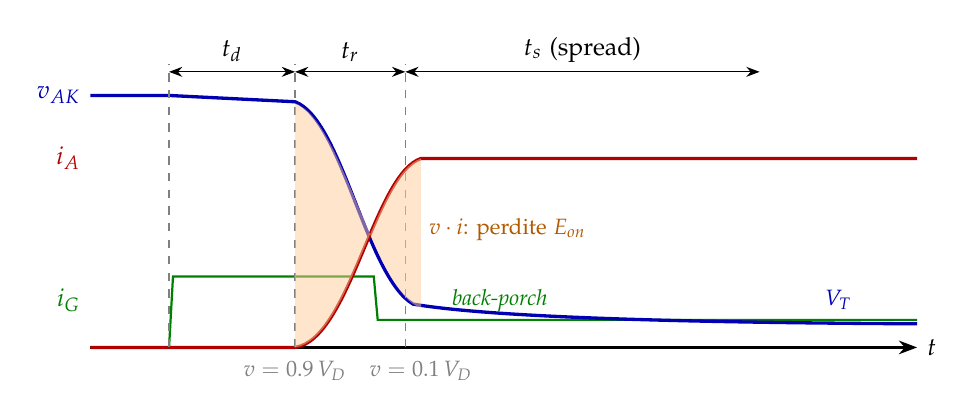
\begin{tikzpicture}[x=1cm,y=1cm,font=\small]
  % axes
  \draw[ax] (0,0) -- (10.5,0) node[right] {$t$};
  % gate current
  \draw[thick,green!50!black] (0,0.0) -- (1.0,0.0) -- (1.05,0.9) -- (3.6,0.9) -- (3.65,0.35) -- (10.5,0.35);
  \node[green!50!black,left] at (0,0.6) {$i_G$};
  \node[green!50!black,font=\footnotesize] at (5.2,0.6) {\en{back-porch}};
  % v_AK
  \draw[very thick,blue!70!black] (0,3.2) -- (1.0,3.2) -- (2.6,3.12) .. controls (3.2,2.9) and (3.5,0.9) .. (4.1,0.55) .. controls (5,0.4) and (7,0.32) .. (10.5,0.3);
  \node[blue!70!black,left] at (0,3.2) {$v_{AK}$};
  \node[blue!70!black,font=\footnotesize] at (9.5,0.6) {$V_T$};
  % i_A
  \draw[very thick,red!70!black] (0,0) -- (2.6,0) .. controls (3.3,0.1) and (3.6,2.2) .. (4.2,2.4) -- (10.5,2.4);
  \node[red!70!black,left] at (0,2.4) {$i_A$};
  % markers
  \draw[dashed,gray] (1.0,0) -- (1.0,3.6);
  \draw[dashed,gray] (2.6,0) -- (2.6,3.6);
  \draw[dashed,gray] (4.0,0) -- (4.0,3.6);
  \draw[dim] (1.0,3.5) -- (2.6,3.5) node[midway,above] {$t_d$};
  \draw[dim] (2.6,3.5) -- (4.0,3.5) node[midway,above] {$t_r$};
  \draw[dim] (4.0,3.5) -- (8.5,3.5) node[midway,above] {$t_s$ (spread)};
  \node[font=\footnotesize,gray] at (2.6,-0.3) {$v=0.9\,V_D$};
  \node[font=\footnotesize,gray] at (4.2,-0.3) {$v=0.1\,V_D$};
  % loss shading
  \fill[orange!40,opacity=0.5] (2.6,0) .. controls (3.3,0.1) and (3.6,2.2) .. (4.2,2.4) -- (4.2,0.5) .. controls (3.6,0.7) and (3.2,2.9) .. (2.6,3.1) -- cycle;
  \node[orange!70!black,font=\footnotesize] at (5.3,1.5) {$v\cdot i$: perdite $E_{on}$};
\end{tikzpicture}
\caption{Forme d'onda qualitative all'accensione con carico resistivo: ritardo $t_d$, salita $t_r$ e fase di \en{spread} in cui la tensione converge lentamente a $V_T$. La zona ombreggiata indica dove si concentrano le perdite di accensione.}
\label{fig:turnon}
\end{figure}

\subsection{Propagazione del plasma e limite di \texorpdfstring{$\didt$}{di/dt}}
\label{sec:spreading}
L'innesco è un fenomeno locale: parte dall'area di emettitore adiacente al gate, dove la densità di corrente di gate è massima, e si propaga lateralmente per diffusione dei portatori nelle basi e per la caduta di tensione laterale che polarizza progressivamente le zone vicine (Fig.~\ref{fig:spread}a). La velocità di propagazione (\en{plasma spreading velocity}) è dell'ordine di
\begin{equation}
  v_s \approx \qtyrange{0.03}{0.1}{\mm\per\us},
\end{equation}
crescente con la densità di corrente e con il tempo di vita dei portatori, decrescente con lo spessore della base n. Per un catodo di raggio \qty{40}{\mm} servono quindi centinaia di microsecondi per l'accensione completa.

La conseguenza è il limite di $\didt$: se il circuito impone una salita di corrente più rapida della crescita dell'area accesa, la densità di corrente nell'area iniziale (pochi \unit{\mm\squared}) diventa enorme, con densità di potenza locale ($J\cdot E$ con tensione ancora elevata) sufficiente a fondere il silicio. I \en{data sheet} specificano ($\didt$)$_{cr}$, tipicamente \qtyrange{100}{1000}{\A\per\us}, in condizioni definite di corrente di gate. Le contromisure sono di due tipi:
\begin{itemize}
  \item \textbf{di circuito}: induttanza di limitazione in serie (spesso saturabile, per non penalizzare la conduzione), \en{snubber} con resistenza sufficiente a limitare la corrente di scarica del condensatore, \en{hard gate drive};
  \item \textbf{di dispositivo}: aumentare la lunghezza del perimetro di gate, cioè la linea da cui parte la propagazione. Da qui i gate interdigitati (\en{involute}, \en{snowflake}) e il gate amplificatore.
\end{itemize}

\subsection{Gate amplificatore}
Nel gate amplificatore (Fig.~\ref{fig:spread}b) il contatto esterno di gate innesca un piccolo tiristore pilota di area ridotta e alta sensibilità, il cui ``catodo'' non è collegato al terminale K ma a una metallizzazione flottante che si sovrappone alla base p in prossimità del catodo principale. La corrente di anodo del pilota (alcune decine di ampere, limitata dalla sua area e dalla resistenza della base) diventa corrente di gate per il tiristore principale lungo tutto il perimetro della metallizzazione flottante. Si ottiene così un innesco di grande area con una corrente esterna di poche centinaia di milliampere, con $t_d$ ridotto e ($\didt$)$_{cr}$ molto più alto. Il pilota è protetto dalla sua stessa corrente perché, una volta acceso il principale, la tensione crolla e il pilota si spegne (la corrente si redistribuisce verso il catodo principale, che ha caduta minore).

\begin{figure}[htbp]
\centering
\begin{subfigure}[b]{0.40\textwidth}
\centering
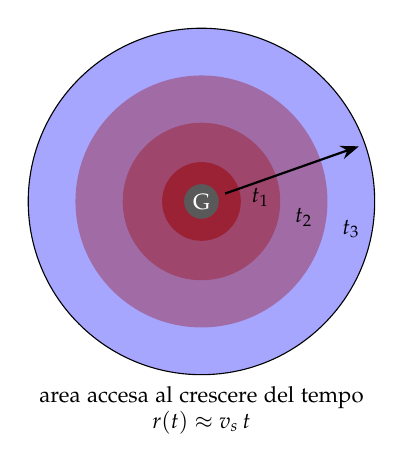
\begin{tikzpicture}[x=1cm,y=1cm,font=\small]
  \fill[layerNp] (0,0) circle (2.2);
  \draw (0,0) circle (2.2);
  \fill[red!60!black,opacity=0.35] (0,0) circle (1.6);
  \fill[red!60!black,opacity=0.35] (0,0) circle (1.0);
  \fill[red!60!black,opacity=0.5] (0,0) circle (0.5);
  \fill[metal] (0,0) circle (0.22);
  \node[white,font=\footnotesize] at (0,0) {G};
  \draw[->,>=Stealth,thick] (0.3,0.1) -- (2.0,0.7);
  \node[font=\footnotesize] at (0.75,0.05) {$t_1$};
  \node[font=\footnotesize] at (1.3,-0.2) {$t_2$};
  \node[font=\footnotesize] at (1.9,-0.35) {$t_3$};
  \node[font=\footnotesize,align=center] at (0,-2.65) {area accesa al crescere del tempo\\ $r(t)\approx v_s\,t$};
\end{tikzpicture}
\caption{vista dall'alto, gate centrale}
\end{subfigure}
\hfill
\begin{subfigure}[b]{0.56\textwidth}
\centering
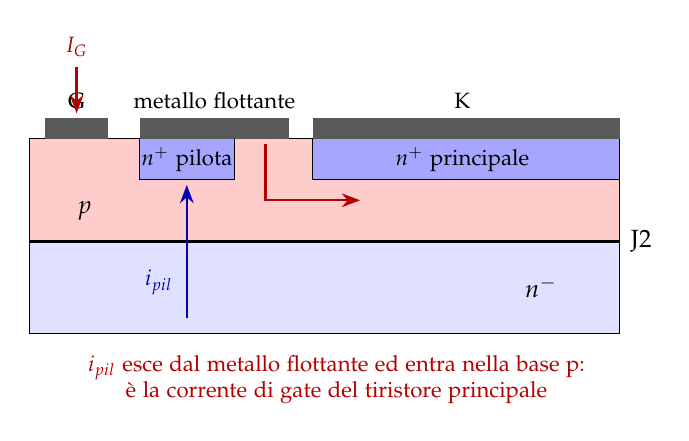
\begin{tikzpicture}[x=1cm,y=1.3cm,font=\small]
  \fill[layerN]  (0,0) rectangle (7.5,0.9);
  \fill[layerP]  (0,0.9) rectangle (7.5,1.9);
  % pilot n+ and main n+
  \fill[layerNp] (1.4,1.5) rectangle (2.6,1.9);
  \fill[layerNp] (3.6,1.5) rectangle (7.5,1.9);
  \draw (0,0) rectangle (7.5,1.9);
  \draw (1.4,1.5) rectangle (2.6,1.9);
  \draw (3.6,1.5) rectangle (7.5,1.9);
  \node at (0.7,1.2) {$p$}; \node at (6.5,0.45) {$n^-$};
  \node[font=\footnotesize] at (2.0,1.7) {$n^+$ pilota};
  \node[font=\footnotesize] at (5.5,1.7) {$n^+$ principale};
  % metallisations
  \fill[metal] (0.2,1.9) rectangle (1.0,2.1);    % gate contact on p
  \fill[metal] (1.4,1.9) rectangle (3.3,2.1);    % floating metal: pilot cathode + p overlap
  \fill[metal] (3.6,1.9) rectangle (7.5,2.1);    % main cathode
  \node[above,font=\footnotesize] at (0.6,2.1) {G};
  \node[above,font=\footnotesize] at (2.35,2.1) {metallo flottante};
  \node[above,font=\footnotesize] at (5.5,2.1) {K};
  \draw[junc] (0,0.9) -- (7.5,0.9) node[right] {J2};
  % currents
  \draw[->,>=Stealth,thick,red!70!black] (0.6,2.6) -- (0.6,2.15);
  \node[red!70!black,font=\footnotesize] at (0.6,2.8) {$\IG$};
  \draw[->,>=Stealth,thick,blue!70!black] (2.0,0.15) -- (2.0,1.45);
  \node[blue!70!black,font=\footnotesize,left] at (1.95,0.5) {$i_{pil}$};
  \draw[->,>=Stealth,thick,red!70!black] (3.0,1.85) -- (3.0,1.3) -- (4.2,1.3);
  \node[red!70!black,font=\footnotesize,align=center] at (3.9,-0.45) {$i_{pil}$ esce dal metallo flottante ed entra nella base p:\\ è la corrente di gate del tiristore principale};
\end{tikzpicture}
\caption{gate amplificatore (sezione)}
\end{subfigure}
\caption{Propagazione laterale del plasma dal gate e struttura a gate amplificatore: il tiristore pilota converte una piccola corrente esterna in una forte corrente di gate distribuita sul perimetro del catodo principale.}
\label{fig:spread}
\end{figure}

% =====================================================================
\section{Stato di conduzione}
% =====================================================================
\subsection{Il plasma nella base n}
In conduzione tutte e tre le giunzioni sono polarizzate direttamente. L'emettitore $p^+$ inietta lacune nella base $n^-$ e l'emettitore $n^+$ inietta elettroni nella base p, che li trasmette (attraverso J2, ora diretta) alla base $n^-$. La base $n^-$ si riempie di un plasma di elettroni e lacune di concentrazione $n\approx p$ molto superiore al drogaggio ($\numrange{e16}{e17}\;\unit{\per\cm\cubed}$ contro $N_D\approx\qty{e13}{\per\cm\cubed}$): è il regime di \emph{alta iniezione} (\en{high-level injection}), lo stesso del diodo PIN. La neutralità di carica impone $n\approx p$ e il profilo è governato dall'equazione di diffusione ambipolare
\begin{equation}
  D_a\,\frac{\dd^2 p}{\dd x^2} = \frac{p}{\tau_{HL}}, \qquad
  D_a = \frac{2D_nD_p}{D_n+D_p}, \qquad L_a = \sqrt{D_a\tau_{HL}},
  \label{eq:ambipolare}
\end{equation}
la cui soluzione è una combinazione di $\cosh$ e $\sinh$ (profilo ``a catenaria'', Fig.~\ref{fig:plasma}): la concentrazione è massima alle due estremità, dove i due emettitori iniettano, e minima al centro. Il rapporto fra i due massimi dipende dal rapporto delle mobilità e dalle efficienze degli emettitori. Nel tiristore, a differenza del diodo, anche la base p è in alta iniezione (elettroni iniettati da J3 in concentrazione confrontabile con $N_A$), il che rende J2 trasparente ai portatori.

\begin{figure}[htbp]
\centering
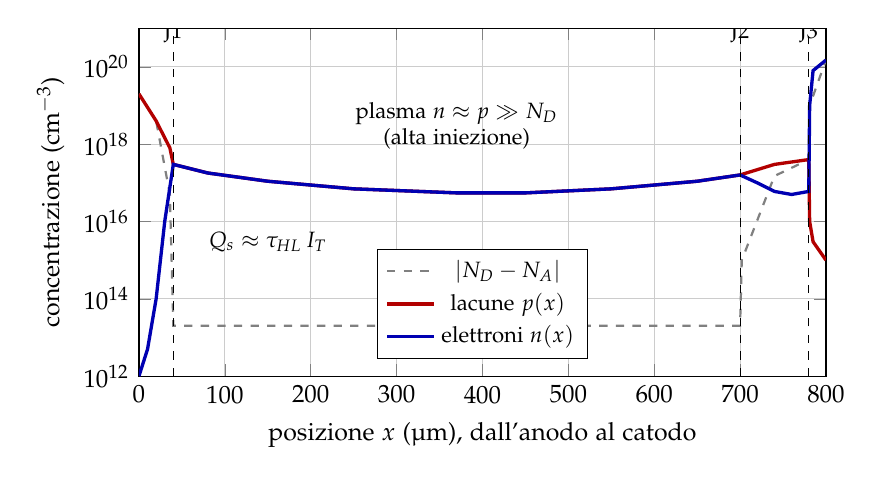
\begin{tikzpicture}
\begin{axis}[
  width=0.85\textwidth, height=6cm,
  xlabel={posizione $x$ (\unit{\um}), dall'anodo al catodo},
  ylabel={concentrazione (\unit{\per\cm\cubed})},
  ymode=log, ymin=1e12, ymax=1e21, xmin=0, xmax=800,
  grid=both, minor grid style={gray!15}, major grid style={gray!40},
  font=\small, ytick={1e12,1e14,1e16,1e18,1e20},
  legend style={font=\footnotesize,at={(0.5,0.05)},anchor=south},
]
% drogaggio (grigio)
\addplot[gray,thick,dashed] coordinates {(0,2e19) (20,4e18) (36,5e16) (40,2e13) (700,2e13) (702,1e15) (740,1.5e17) (780,4e17) (781,1e19) (800,1.5e20)};
\addlegendentry{$|N_D-N_A|$}
% lacune
\addplot[red!70!black,very thick] coordinates {(0,2e19) (20,4e18) (36,8e17) (40,3e17) (80,1.8e17) (150,1.1e17) (250,7e16) (370,5.5e16) (450,5.5e16) (550,7e16) (650,1.1e17) (700,1.6e17) (740,3e17) (780,4e17) (781,1e16) (785,3e15) (800,1e15)};
\addlegendentry{lacune $p(x)$}
% elettroni
\addplot[blue!70!black,very thick] coordinates {(0,1e12) (10,5e12) (20,1e14) (30,1e16) (40,3e17) (80,1.8e17) (150,1.1e17) (250,7e16) (370,5.5e16) (450,5.5e16) (550,7e16) (650,1.1e17) (700,1.6e17) (720,1.0e17) (740,6e16) (760,5e16) (780,6e16) (781,1e19) (785,8e19) (800,1.5e20)};
\addlegendentry{elettroni $n(x)$}
\draw[dashed] (axis cs:40,1e12) -- (axis cs:40,1e21) node[above,pos=0.93,font=\footnotesize] {J1};
\draw[dashed] (axis cs:700,1e12) -- (axis cs:700,1e21) node[above,pos=0.93,font=\footnotesize] {J2};
\draw[dashed] (axis cs:780,1e12) -- (axis cs:780,1e21) node[above,pos=0.93,font=\footnotesize] {J3};
\node[font=\footnotesize,align=center] at (axis cs:370,3e18) {plasma $n\approx p \gg N_D$\\ (alta iniezione)};
\node[font=\footnotesize] at (axis cs:150,3e15) {$Q_s \approx \tau_{HL}\,I_T$};
\end{axis}
\end{tikzpicture}
\caption{Profilo qualitativo dei portatori in conduzione: la base $n^-$ è inondata da un plasma quasi neutro con profilo a catenaria; la base p è anch'essa in alta iniezione. La carica immagazzinata $Q_s$ è quella che va rimossa allo spegnimento.}
\label{fig:plasma}
\end{figure}

\subsection{Caduta di tensione diretta}
Percorrendo il dispositivo da anodo a catodo la tensione totale è
\begin{equation}
  V_T = V_{J1} - V_{J2} + V_{J3} + V_{N} + V_{P} + V_{cont},
  \label{eq:VT}
\end{equation}
dove $V_{J2}$ compare con segno negativo perché J2 è orientata in senso opposto: le tre giunzioni sono tutte polarizzate direttamente, ma J2 sottrae anziché aggiungere. Il risultato netto delle tre giunzioni è dell'ordine di una sola caduta di giunzione (\qtyrange{0.8}{1.0}{\V}), a cui si aggiunge la caduta ohmica $V_N$ nella base n modulata dal plasma. Come nel diodo PIN, in alta iniezione la conduttività della base è $\sigma = q(\mu_n+\mu_p)p$ e la caduta $V_N$ diventa indipendente dalla corrente:
\begin{equation}
  V_N \approx \frac{W_N^2}{(\mu_n+\mu_p)\,\tau_{HL}}\quad(\text{per } W_N \lesssim 2L_a),
\end{equation}
il che spiega perché la caratteristica di conduzione sia quasi una retta con pendenza modesta e perché il tempo di vita $\tau_{HL}$ sia il parametro che scambia $V_T$ contro velocità di spegnimento (\S\ref{sec:lifetime}). Per basi molto spesse ($W_N\gg L_a$) il plasma non riesce a riempire il centro della base e $V_N$ cresce esponenzialmente con $W_N/L_a$. I \en{data sheet} riportano la caratteristica diretta con il modello lineare
\begin{equation}
  V_T(I_T) = V_{T0} + r_T\,I_T,
\end{equation}
con $V_{T0}\approx\qtyrange{0.9}{1.3}{\V}$ e $r_T$ di frazioni di \unit{\milli\ohm} per dispositivi da migliaia di ampere, usato per il calcolo delle perdite di conduzione $P = V_{T0}I_{TAV} + r_T I_{TRMS}^2$. A parità di area, $V_T$ cresce con la classe di tensione perché cresce $W_N$: circa \qty{1.2}{\V} a \qty{1.6}{\kV}, \qtyrange{1.8}{2.5}{\V} a \qtyrange{6.5}{8.5}{\kV} alla corrente nominale.

In conduzione il gate non ha alcuna influenza: la corrente di base di $Q_2$ arriva interamente dal collettore di $Q_1$ e una corrente di gate negativa di entità ragionevole (in un SCR convenzionale) viene semplicemente deviata dalla base p senza interrompere la rigenerazione, perché la base p è allagata da portatori e ha resistenza laterale troppo bassa per polarizzare inversamente J3 su tutta l'area. Il GTO è il dispositivo in cui la geometria del catodo (\en{fingers} stretti, nessun \en{short}) è progettata proprio per rendere possibile questo spegnimento da gate.

\subsection{Caratteristica statica completa}
La Fig.~\ref{fig:IV} riassume i tre stati nel piano $I$--$V$. Il ramo di blocco diretto termina in $\VBO$ (corrente di gate nulla) e, con corrente di gate crescente, $\VBO$ si abbassa fino a scomparire: per $\IG\geq I_{GT}$ la caratteristica è quella di un diodo. Il tratto a resistenza negativa fra blocco e conduzione non è osservabile staticamente (è instabile) e corrisponde al transitorio di innesco. Sul ramo di conduzione, riducendo la corrente si scende fino a $\IH$, sotto la quale il dispositivo torna in blocco. In inverso la caratteristica è quella del diodo J1: leakage fino a $V_{BR}$ e poi valanga.

\begin{figure}[htbp]
\centering
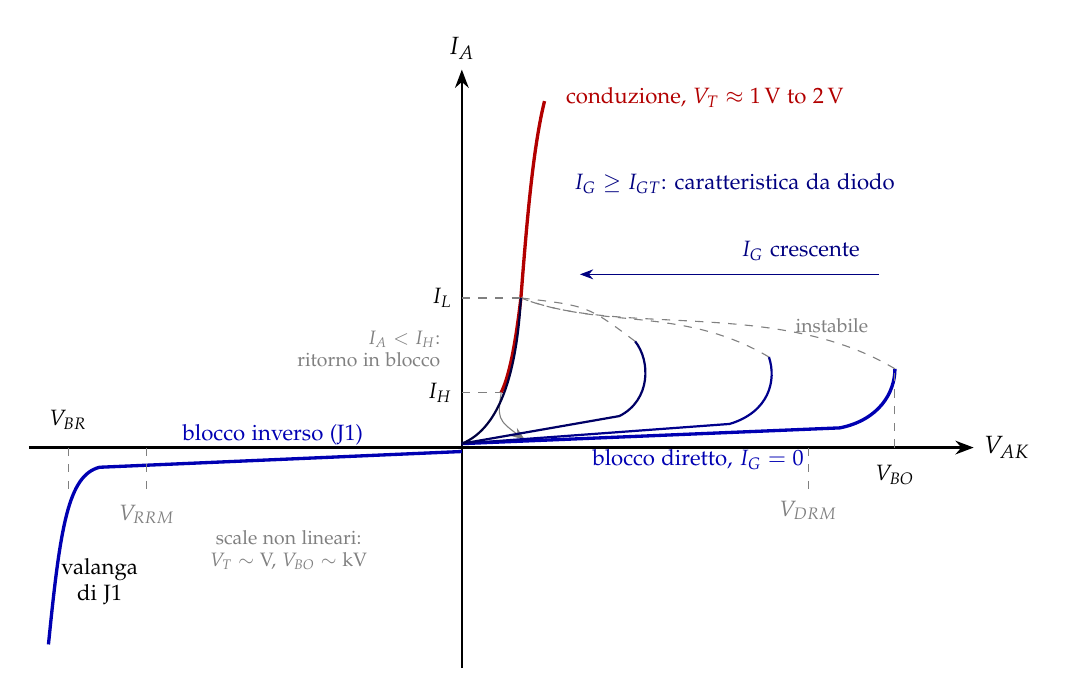
\begin{tikzpicture}[x=1cm,y=1cm,font=\small]
  \draw[ax] (-5.5,0) -- (6.5,0) node[right] {$\VAK$};
  \draw[ax] (0,-2.8) -- (0,4.8) node[above] {$\IA$};
  % --- conduzione ---
  \draw[very thick,red!70!black] (0.75,1.9) .. controls (0.82,2.8) and (0.9,3.8) .. (1.05,4.4);
  \draw[very thick,red!70!black] (0.75,1.9) .. controls (0.68,1.3) and (0.6,0.9) .. (0.5,0.7);
  \node[red!70!black,font=\footnotesize,right] at (1.2,4.45) {conduzione, $V_T\approx\qtyrange{1}{2}{\V}$};
  \draw[dashed,gray] (0,0.7) -- (0.5,0.7); \node[left,font=\footnotesize] at (0,0.7) {$\IH$};
  \draw[dashed,gray] (0,1.9) -- (0.75,1.9); \node[left,font=\footnotesize] at (0,1.9) {$\IL$};
  \draw[->,>=Stealth,gray] (0.5,0.7) .. controls (0.45,0.35) .. (0.8,0.1);
  \node[gray,font=\scriptsize,left,align=right] at (-0.15,1.25) {$\IA<\IH$:\\ ritorno in blocco};
  % --- blocco diretto, IG = 0 ---
  \draw[very thick,blue!70!black] (0,0.05) -- (4.8,0.25) .. controls (5.3,0.35) and (5.5,0.7) .. (5.5,1.0);
  \draw[dashed,gray] (5.5,1.0) .. controls (4.0,1.9) and (2.0,1.4) .. (0.75,1.9);
  \node[blue!70!black,font=\footnotesize,below] at (3.0,0.1) {blocco diretto, $\IG=0$};
  \draw[dashed,gray] (5.5,0) -- (5.5,1.0);
  \node[font=\footnotesize] at (5.5,-0.35) {$\VBO$};
  \draw[dashed,gray] (4.4,0) -- (4.4,-0.55);
  \node[font=\footnotesize,gray] at (4.4,-0.8) {$\VDRM$};
  % --- IG1 > 0 ---
  \draw[thick,blue!55!black] (0,0.05) -- (3.4,0.3) .. controls (3.9,0.45) and (4.0,0.85) .. (3.9,1.15);
  \draw[dashed,gray] (3.9,1.15) .. controls (2.8,1.8) and (1.8,1.5) .. (0.75,1.9);
  % --- IG2 > IG1 ---
  \draw[thick,blue!40!black] (0,0.05) -- (2.0,0.4) .. controls (2.4,0.6) and (2.4,1.1) .. (2.2,1.35);
  \draw[dashed,gray] (2.2,1.35) .. controls (1.6,1.8) .. (0.75,1.9);
  % --- IG >= IGT: diodo ---
  \draw[thick,blue!25!black] (0,0.05) .. controls (0.5,0.25) and (0.7,1.0) .. (0.75,1.9);
  \node[font=\footnotesize,blue!50!black] at (4.3,2.5) {$\IG$ crescente};
  \draw[->,>=Stealth,blue!50!black] (5.3,2.2) -- (1.5,2.2);
  \node[font=\footnotesize,blue!50!black,align=left,right] at (1.3,3.35) {$\IG\geq I_{GT}$: caratteristica da diodo};
  \node[font=\scriptsize,gray] at (4.7,1.55) {instabile};
  % --- blocco inverso ---
  \draw[very thick,blue!70!black] (0,-0.05) -- (-4.6,-0.25) .. controls (-5.0,-0.35) and (-5.1,-1.0) .. (-5.25,-2.5);
  \node[blue!70!black,font=\footnotesize,above] at (-2.4,-0.1) {blocco inverso (J1)};
  \draw[dashed,gray] (-5.0,0) -- (-5.0,-0.6); \node[font=\footnotesize] at (-5.0,0.35) {$V_{BR}$};
  \draw[dashed,gray] (-4.0,0) -- (-4.0,-0.6); \node[font=\footnotesize,gray] at (-4.0,-0.85) {$\VRRM$};
  \node[font=\footnotesize,align=center] at (-4.6,-1.7) {valanga\\ di J1};
  \node[font=\scriptsize,gray,align=center] at (-2.2,-1.3) {scale non lineari:\\ $V_T\sim$ V, $\VBO\sim$ kV};
\end{tikzpicture}
\caption{Caratteristica statica $I$--$V$ del tiristore. Il ramo a resistenza negativa (tratteggiato) è instabile; la corrente di gate abbassa la tensione di \en{breakover} fino a rendere il dispositivo equivalente a un diodo.}
\label{fig:IV}
\end{figure}

% =====================================================================
\section{Spegnimento}
% =====================================================================
\subsection{Reverse recovery}
\label{sec:rr}
Il tiristore convenzionale non può essere spento dal gate: lo spegnimento avviene quando il circuito esterno riduce la corrente sotto $\IH$, per commutazione naturale (inversione della tensione di rete nei convertitori a commutazione di rete) o forzata (circuito risonante o di commutazione ausiliaria). Il processo (Fig.~\ref{fig:turnoff}) è quello del \en{reverse recovery} del diodo PIN, complicato dalla presenza della terza giunzione:
\begin{enumerate}
  \item La corrente decresce con pendenza $-\didt$ imposta dal circuito (per esempio $V/L_{comm}$). Finché nella base n c'è plasma, il dispositivo resta a bassa impedenza e la corrente prosegue nel verso inverso: le lacune del plasma vengono estratte verso l'anodo, gli elettroni verso il catodo.
  \item J3 è la prima a recuperare: la sua carica è piccola e, appena la zona adiacente si svuota, si polarizza inversamente e va in valanga a \qtyrange{10}{20}{\V} (oppure è bypassata dagli \en{shorts}): il suo contributo è trascurabile.
  \item J1 recupera quando la concentrazione di plasma al suo bordo si annulla: da quel momento può sostenere tensione inversa, la regione di svuotamento si allarga nella base n estraendo la carica residua e la corrente inversa raggiunge il picco $I_{RM}$ e poi decresce verso zero (fase $t_b$). Con l'induttanza di commutazione la rapida diminuzione della corrente inversa produce una sovratensione $L\,\didt$, contenuta dallo \en{snubber} RC.
  \item Al termine del recupero ($t_{rr}=t_a+t_b$) la corrente è praticamente nulla e il dispositivo sostiene tensione inversa, ma \emph{non è ancora in grado di bloccare tensione diretta}: J2 non ha recuperato e nella metà della base n vicina a J2 e nella base p rimane plasma che può solo ricombinarsi.
\end{enumerate}
La carica di recupero $Q_{rr}=\int i_R\,\dd t$ è una frazione della carica immagazzinata $Q_s\approx\tau_{HL}I_T$ (la parte restante ricombina durante $t_a$ e dopo $t_{rr}$) e cresce con $I_T$, con $T_j$ e con la lentezza del $\didt$. Per un dispositivo di grande area per controllo di fase $Q_{rr}$ è dell'ordine di \qtyrange{1000}{10000}{\micro\coulomb}. Approssimando la forma d'onda inversa con un triangolo di \en{softness} $S=t_b/t_a$:
\begin{equation}
  Q_{rr} \approx \tfrac12 I_{RM}\,t_{rr}, \qquad
  I_{RM} \approx \sqrt{\frac{2\,Q_{rr}\,(\didt)}{1+S}}, \qquad
  t_a = \frac{I_{RM}}{\didt}.
\end{equation}
L'energia dissipata nel recupero è $E_{rr}\approx\int v_{AK}\,i\,\dd t$ durante $t_b$, quando tensione inversa e corrente inversa coesistono; nei convertitori a commutazione di rete a \qty{50}{\Hz} è piccola rispetto alle perdite di conduzione, ma diventa significativa nei tiristori veloci a frequenza di commutazione più alta.

\begin{figure}[htbp]
\centering
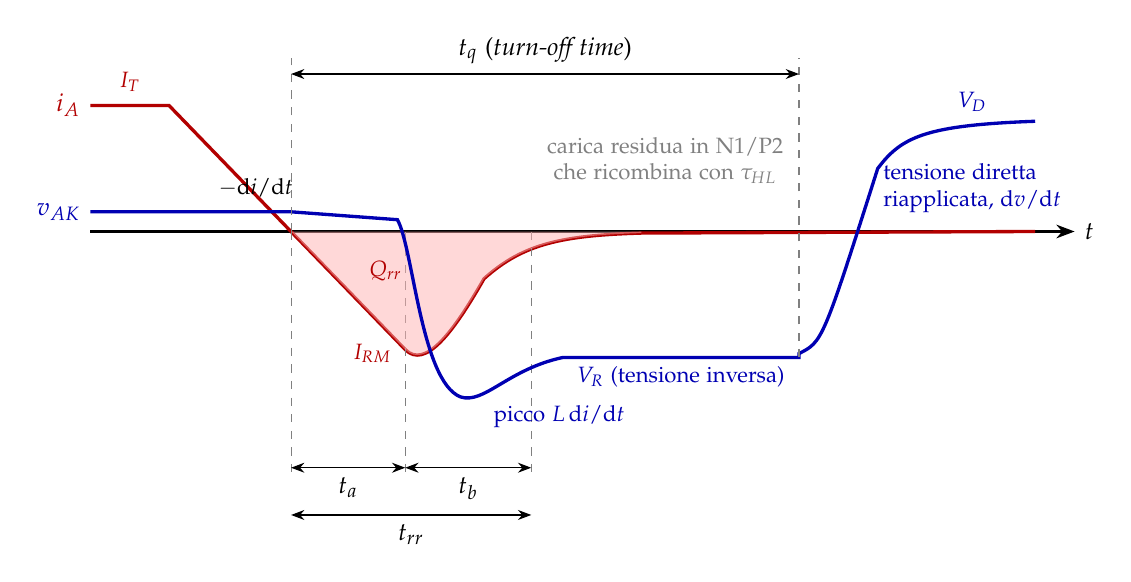
\begin{tikzpicture}[x=1cm,y=1cm,font=\small]
  % time axis
  \draw[ax] (0,0) -- (12.5,0) node[right] {$t$};
  % current
  \draw[very thick,red!70!black] (0,1.6) -- (1.0,1.6) -- (4.0,-1.5) .. controls (4.25,-1.75) and (4.6,-1.3) .. (5.0,-0.6) .. controls (5.5,-0.15) and (6,-0.05) .. (7,-0.02) -- (12,0);
  \node[red!70!black,left] at (0,1.6) {$i_A$};
  \node[red!70!black,font=\footnotesize] at (0.5,1.9) {$I_T$};
  \node[font=\footnotesize] at (2.1,0.55) {$-\didt$};
  \draw[dashed,gray] (2.55,0) -- (2.55,-3.1);
  \draw[dashed,gray] (4.0,0) -- (4.0,-3.1);
  \draw[dashed,gray] (5.6,0) -- (5.6,-3.1);
  \draw[dim] (2.55,-3.0) -- (4.0,-3.0) node[midway,below] {$t_a$};
  \draw[dim] (4.0,-3.0) -- (5.6,-3.0) node[midway,below] {$t_b$};
  \node[red!70!black,font=\footnotesize,left] at (3.95,-1.55) {$I_{RM}$};
  \fill[red!30,opacity=0.5] (2.55,0) -- (4.0,-1.5) .. controls (4.25,-1.75) and (4.6,-1.3) .. (5.0,-0.6) .. controls (5.5,-0.15) and (6,-0.05) .. (7,-0.02) -- (7,0) -- cycle;
  \node[red!70!black,font=\footnotesize] at (3.75,-0.5) {$Q_{rr}$};
  % voltage
  \draw[very thick,blue!70!black] (0,0.25) -- (2.55,0.25) -- (3.9,0.15) .. controls (4.1,-0.2) and (4.2,-1.9) .. (4.7,-2.1) .. controls (5.0,-2.2) and (5.3,-1.75) .. (6.0,-1.6) -- (9.0,-1.6) -- (9.0,-1.55) .. controls (9.3,-1.4) .. (10.0,0.8) .. controls (10.3,1.2) and (10.6,1.35) .. (12,1.4);
  \node[blue!70!black,left] at (0,0.25) {$v_{AK}$};
  \node[blue!70!black,font=\footnotesize,right] at (5.0,-2.35) {picco $L\,\didt$};
  \node[blue!70!black,font=\footnotesize] at (7.5,-1.85) {$V_R$ (tensione inversa)};
  \node[blue!70!black,font=\footnotesize,align=left] at (11.2,0.55) {tensione diretta\\ riapplicata, $\dvdt$};
  \node[blue!70!black,font=\footnotesize] at (11.2,1.65) {$V_D$};
  % tq
  \draw[dashed,gray] (9.0,-1.6) -- (9.0,2.2);
  \draw[dashed,gray] (2.55,0) -- (2.55,2.2);
  \draw[dim] (2.55,2.0) -- (9.0,2.0) node[midway,above] {$\tq$ (\en{turn-off time})};
  \draw[dim] (2.55,-3.6) -- (5.6,-3.6) node[midway,below] {$t_{rr}$};
  % residual charge note
  \node[font=\footnotesize,gray,align=center] at (7.3,0.9) {carica residua in N1/P2\\ che ricombina con $\tau_{HL}$};
\end{tikzpicture}
\caption{Forme d'onda qualitative allo spegnimento per commutazione naturale: \en{reverse recovery} ($t_a$, $t_b$, $I_{RM}$, $Q_{rr}$), tensione inversa, e tempo di \en{turn-off} $\tq$ misurato dal passaggio per lo zero della corrente alla riapplicazione della tensione diretta.}
\label{fig:turnoff}
\end{figure}

\subsection{Tempo di turn-off \texorpdfstring{$\tq$}{tq}}
Il parametro dinamico caratteristico del tiristore è $\tq$: il tempo minimo che deve trascorrere dal passaggio per lo zero della corrente di anodo alla riapplicazione della tensione diretta perché il dispositivo \emph{non} si riaccenda. Il meccanismo è il seguente: dopo il recupero di J1, nella base n vicina a J2 e nella base p rimane un plasma residuo che decade per ricombinazione con costante di tempo $\tau_{HL}$ (nessuna corrente lo estrae, perché J1 blocca). Se si riapplica tensione diretta, J2 deve svuotarsi: i portatori residui vengono spazzati via dal campo che si forma e costituiscono una corrente attraverso J2 che, ancora una volta, è corrente di base per entrambi i transistori. Si somma a essa la corrente capacitiva $C_{J2}\,\dvdt$. Se la carica residua è ancora sufficiente perché $\alpha_1+\alpha_2$ raggiunga uno, il tiristore si riaccende senza comando di gate (\en{commutation failure}). In prima approssimazione la carica residua decade come $Q(t)=Q_0 e^{-t/\tau_{HL}}$ e
\begin{equation}
  \tq \approx \tau_{HL}\ln\frac{Q_0}{Q_{crit}} \approx (\numrange{3}{6})\,\tau_{HL},
\end{equation}
con $Q_{crit}$ la carica che, spazzata via da J2 alla riapplicazione, produce la corrente di innesco. Ne segue che $\tq$:
\begin{itemize}
  \item cresce con $T_j$ (aumentano $\tau_{HL}$ e i guadagni; il valore di \en{data sheet} è a $T_{j,max}$);
  \item cresce con la corrente $I_T$ prima dello spegnimento e diminuisce con $\didt$ (più carica estratta nel recupero);
  \item cresce con il $\dvdt$ e con la tensione $V_D$ riapplicati, e diminuisce se durante l'intervallo è applicata una tensione inversa maggiore (si mantiene J1 in blocco con svuotamento più profondo);
  \item cresce con lo spessore della base n, cioè con la classe di tensione.
\end{itemize}
Nei convertitori a commutazione di rete in funzionamento da inverter, $\tq$ fissa l'angolo di estinzione minimo $\gamma_{min} = \omega\,\tq + \text{margine}$: con $\tq=\qty{400}{\us}$ a \qty{50}{\Hz}, $\omega\tq \approx \ang{7.2}$, a cui si aggiungono l'angolo di sovrapposizione e un margine per le variazioni di rete (da cui i tipici $\gamma\approx\ang{15}$--$\ang{18}$ dei collegamenti HVDC-LCC). Nei circuiti a commutazione forzata $\tq$ determina direttamente il dimensionamento del condensatore di commutazione e la frequenza massima.

\subsection{Controllo del tempo di vita: phase-control vs fast thyristor}
\label{sec:lifetime}
Tutti i parametri dinamici ($Q_{rr}$, $I_{RM}$, $\tq$) scalano con $\tau_{HL}$, ma anche la caduta $V_T$ e, in misura minore, il leakage e $\IH$ dipendono da esso in senso opposto: ridurre $\tau_{HL}$ rende il dispositivo più veloce ma con perdite di conduzione più alte. La tecnologia sceglie il compromesso:
\begin{itemize}
  \item i \textbf{tiristori per controllo di fase} (\en{phase-control}, PCT) hanno $\tau_{HL}$ lungo (decine o centinaia di \unit{\us}), la minima $V_T$ e $\tq$ di \qtyrange{100}{700}{\us}: sono ottimizzati per la conduzione a \qty{50}{\Hz}/\qty{60}{\Hz};
  \item i \textbf{tiristori veloci} (\en{fast}, \en{inverter-grade}) hanno $\tau_{HL}$ ridotto artificialmente a pochi \unit{\us} con diffusione di oro o platino (centri di ricombinazione profondi) oppure con irraggiamento di elettroni o protoni (difetti puntuali, con controllo anche del profilo locale), ottenendo $\tq=\qtyrange{5}{50}{\us}$ a costo di $V_T$ maggiore del \qtyrange{30}{100}{\percent}. L'irraggiamento è preferito perché più riproducibile, con minore impatto sul leakage e con la possibilità di ricottura selettiva.
\end{itemize}
La stessa leva di progetto, combinata con la struttura asimmetrica e un catodo interdigitato senza \en{shorts}, porta al GTO e poi all'IGCT, in cui il tempo di vita è ottimizzato per uno spegnimento controllato da gate a guadagno unitario.

% =====================================================================
\section{Parametri di data sheet e loro origine fisica}
% =====================================================================
La Tab.~\ref{tab:params} collega i principali parametri specificati dai costruttori (IEC 60747-6~\cite{iec60747}) ai fenomeni fisici descritti nei capitoli precedenti. Gli ordini di grandezza si riferiscono a un tiristore \en{press-pack} per controllo di fase nella classe \qtyrange{4.5}{8.5}{\kV}, \qtyrange{2}{5}{\kA}.

\begin{table}[htbp]
\centering\small
\begin{tabular}{@{}>{\raggedright\arraybackslash}p{3.6cm}>{\raggedright\arraybackslash}p{1.7cm}>{\raggedright\arraybackslash}p{3.2cm}>{\raggedright\arraybackslash}p{6.3cm}@{}}
\toprule
Parametro & Simbolo & Ordine di grandezza & Origine fisica \\
\midrule
Tensione ripetitiva di picco diretta/inversa & $\VDRM$, $\VRRM$ & \qtyrange{4.5}{8.5}{\kV} & rottura a valanga di J2/J1 nella base $n^-$, ridotta dai guadagni (eq.~\ref{eq:VBO}) e dalla terminazione di bordo; margine su $\VBO$ \\
Corrente media in conduzione & $I_{TAV}$ & \qtyrange{2}{5}{\kA} & limite termico: $V_{T0}$, $r_T$, $R_{th,jc}$, $T_{j,max}$ \\
Corrente di picco non ripetitiva (\qty{10}{\ms}) & $I_{TSM}$ & \qtyrange{30}{100}{\kA} & fusione locale/limite termico adiabatico; $I^2t$ per il coordinamento con i fusibili \\
Caduta diretta & $V_{T0}$, $r_T$ & \qtyrange{0.9}{1.3}{\V}, \qtyrange{0.1}{0.5}{\milli\ohm} & tre giunzioni + base $n^-$ modulata dal plasma (eq.~\ref{eq:VT}) \\
Corrente di leakage a $\VDRM$, $T_{j,max}$ & $I_{DRM}$, $I_{RRM}$ & \qtyrange{100}{500}{\mA} & generazione nella regione di svuotamento, amplificata da $1/(1-\alpha_1-\alpha_2)$ \\
$\dvdt$ critico & ($\dvdt$)$_{cr}$ & \qtyrange{500}{2000}{\V\per\us} & corrente capacitiva di J2 vs soglia laterale nella base p; \en{cathode shorts} \\
$\didt$ critico & ($\didt$)$_{cr}$ & \qtyrange{100}{1000}{\A\per\us} & velocità di propagazione del plasma; perimetro di gate, gate amplificatore \\
Corrente/tensione di gate di innesco & $I_{GT}$, $V_{GT}$ & \qtyrange{0.1}{0.4}{\A}, \qtyrange{1.5}{3}{\V} & soglia di J3 raggiunta dalla caduta laterale nella base p; \en{shorts} \\
Holding / latching current & $\IH$, $\IL$ & \qtyrange{0.1}{1}{\A} & $\alpha_1+\alpha_2=1$ su tutta l'area / sull'area iniziale \\
Tempo di ritardo, di accensione & $t_d$, $t_{gt}$ & \qtyrange{1}{5}{\us} & tempi di transito in base e riempimento della base n \\
Carica di recupero & $Q_{rr}$ & \qtyrange{1}{10}{\milli\coulomb} & carica immagazzinata $\tau_{HL}I_T$, dipende da $\didt$, $T_j$ \\
Tempo di turn-off & $\tq$ & \qtyrange{100}{700}{\us} & ricombinazione della carica residua in N1/P2 con $\tau_{HL}$ \\
Resistenza termica giunzione--case & $R_{th,jc}$ & \qtyrange{5}{15}{\K\per\kW} & dischi di Mo/W, contatto a pressione doppia faccia \\
\bottomrule
\end{tabular}
\caption{Principali parametri di \en{data sheet} di un tiristore di potenza per controllo di fase e fenomeni fisici da cui dipendono (valori indicativi).}
\label{tab:params}
\end{table}

% =====================================================================
\section{Varianti della struttura base}
% =====================================================================
Le variazioni sulla struttura p-n-p-n nascono tutte dall'agire su uno dei meccanismi descritti:
\begin{description}
  \item[ASCR / RCT] (\en{asymmetric}, \en{reverse conducting}): \en{buffer} $n$ davanti all'emettitore di anodo (\en{field stop}) per accorciare la base n; rinuncia al blocco inverso in cambio di $V_T$, $Q_{rr}$ e $\tq$ minori. Nell'RCT il diodo di libera circolazione è integrato sullo stesso wafer.
  \item[LTT] (\en{light-triggered}): innesco ottico con gate amplificatore a più stadi, per le valvole HVDC.
  \item[BOD / protezione integrata] tiristori con \en{breakover} controllato e riproducibile, usati come protezione da sovratensione (\en{crowbar}, protezione delle valvole).
  \item[GTO] emettitore di catodo frammentato in migliaia di \en{fingers} stretti (\qtyrange{100}{300}{\um}) senza \en{shorts}, anodo con \en{shorts} (\en{anode shorts}) o \en{buffer}: la corrente di gate negativa riesce a spolarizzare J3 su tutta l'area e interrompere la rigenerazione. Guadagno di spegnimento \numrange{3}{5}, spegnimento lento e disomogeneo, necessità di \en{snubber} $\dvdt$.
  \item[IGCT] GTO con \en{hard drive}: unità di gate a bassissima induttanza ($<\qty{5}{\nano\henry}$) che devia allo spegnimento l'intera corrente di anodo nel gate in meno di \qty{1}{\us} (guadagno unitario), trasformando il dispositivo in un p-n-p a base aperta prima che la tensione salga: spegnimento omogeneo senza \en{snubber}, con struttura a \en{buffer} e anodo trasparente.
  \item[Tiristori bidirezionali] (TRIAC, BCT): due strutture p-n-p-n in antiparallelo sullo stesso chip, per correnti alternate a bassa (TRIAC) e alta (BCT) potenza.
\end{description}

% =====================================================================
\section{Conclusioni}
% =====================================================================
Il tiristore si spiega interamente con tre ingredienti della fisica dei semiconduttori: le giunzioni p-n con i loro regimi di iniezione e svuotamento, il guadagno di corrente del transistor bipolare e la sua dipendenza dalla corrente, e la dinamica della carica immagazzinata in una base larga in alta iniezione. La retroazione positiva fra i due transistori interni ($\alpha_1+\alpha_2\to1$) produce la commutazione da blocco a conduzione; l'alta iniezione nella base n produce la bassa caduta a tensioni di blocco di migliaia di volt; la stessa carica immagazzinata, insieme all'assenza di un meccanismo di estrazione controllata, produce il \en{reverse recovery} e il tempo di \en{turn-off} che rendono il tiristore un dispositivo a commutazione naturale. Ogni parametro di \en{data sheet} ($\VBO$, $\dvdt$, $\didt$, $\IH$, $Q_{rr}$, $\tq$) è il riflesso macroscopico di uno di questi meccanismi, e ogni variante (ASCR, LTT, GTO, IGCT) è il risultato di una modifica mirata della struttura che li governa.

% =====================================================================
\begin{thebibliography}{9}
\bibitem{baliga} B.~J. Baliga, \emph{Fundamentals of Power Semiconductor Devices}, 2nd ed. Cham: Springer, 2019, cap.~8 (Thyristors).
\bibitem{lutz} J.~Lutz, H.~Schlangenotto, U.~Scheuermann, and R.~De Doncker, \emph{Semiconductor Power Devices: Physics, Characteristics, Reliability}, 2nd ed. Berlin: Springer, 2018, cap.~8.
\bibitem{mohan} N.~Mohan, T.~M. Undeland, and W.~P. Robbins, \emph{Power Electronics: Converters, Applications, and Design}, 3rd ed. Hoboken, NJ: Wiley, 2003, cap.~23.
\bibitem{sze} S.~M. Sze and K.~K. Ng, \emph{Physics of Semiconductor Devices}, 3rd ed. Hoboken, NJ: Wiley, 2007, cap.~11.
\bibitem{blicher} A.~Blicher, \emph{Thyristor Physics}. New York: Springer, 1976.
\bibitem{ghandhi} S.~K. Ghandhi, \emph{Semiconductor Power Devices}. New York: Wiley, 1977.
\bibitem{gentry} F.~E. Gentry, F.~W. Gutzwiller, N.~Holonyak, and E.~E. Von Zastrow, \emph{Semiconductor Controlled Rectifiers: Principles and Applications of p-n-p-n Devices}. Englewood Cliffs, NJ: Prentice-Hall, 1964.
\bibitem{moll1956} J.~L. Moll, M.~Tanenbaum, J.~M. Goldey, and N.~Holonyak, ``P-N-P-N transistor switches,'' \emph{Proc. IRE}, vol.~44, no.~9, pp.~1174--1182, Sep. 1956.
\bibitem{iec60747} IEC 60747-6, \emph{Semiconductor devices -- Discrete devices -- Part 6: Thyristors}, International Electrotechnical Commission.
\end{thebibliography}

\end{document}
